\section{Stardice response}
\label{sec:rsd}

In this part, we will show how one can obtain the \SD telescope response $\Rtel$ from the Equation~\ref{eq:rsd}. The quantities $\Qccd$ and $\Qphot$ are defined in table \ref{tab:quantities}, and $\Rcbp$ is the CBP response.

\subsection{Data set description}
\label{sec:sd_datadesc}

As described in section \ref{sec:cbp_datadesc}, the laser will still emits pulses at a rate of \SI{1}{\kilo\hertz}. The operational mode is the same, we shoot bursts of pulses that are separated with dark times. We show in Figure~\ref{fig:ccd_examples} examples of images obtained when shooting in the \SD CCD camera. 

\begin{figure}[h]
    \centering
    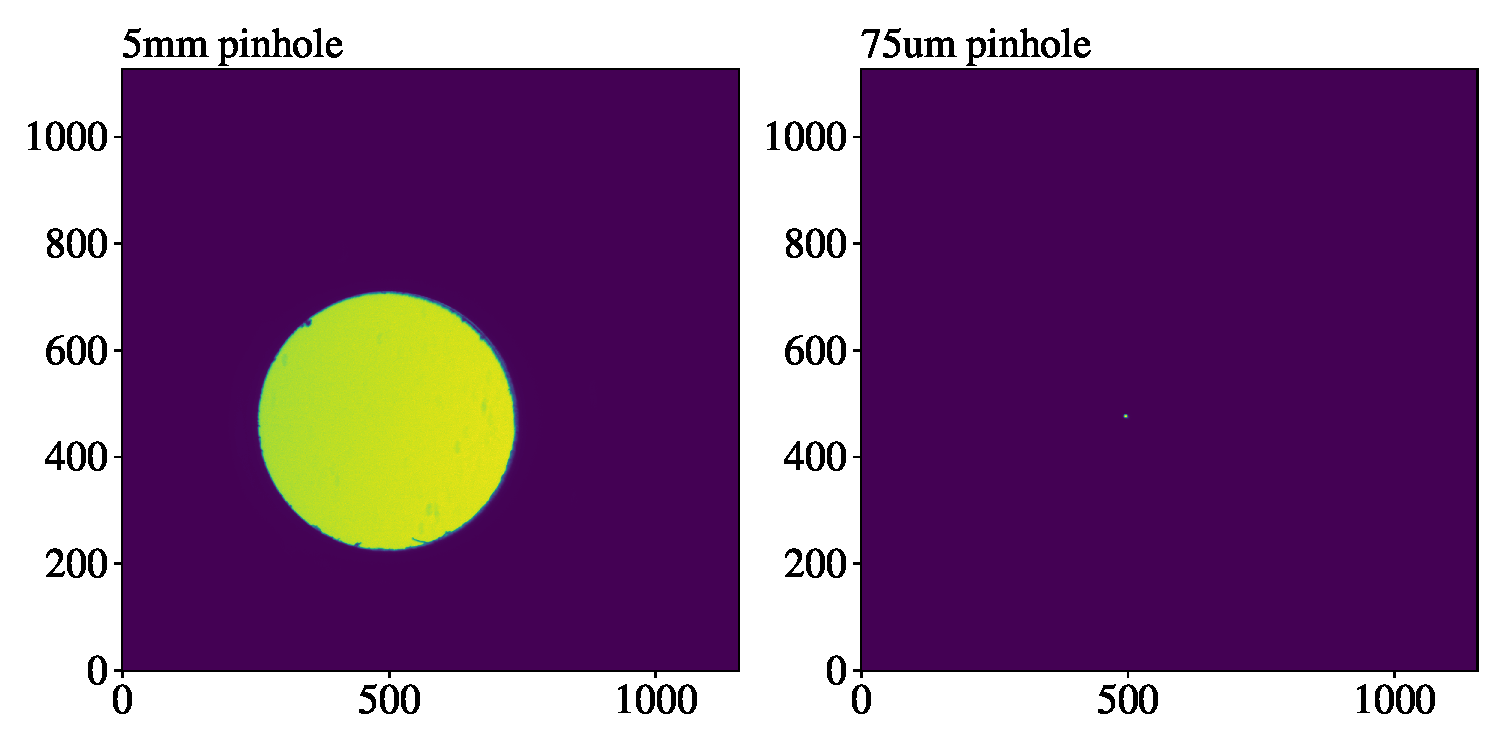
\includegraphics[width=\columnwidth]{fig/ccd_examples.pdf}
    \caption{Examples of images obtained when shooting in the \SD telescope with the CBP at \SI{450}{\nm}. From left to right, we have respectively an image for the \SI{5}{\mm}, \SI{2}{\mm} and \SI{75}{\micro\meter} pinhole.}
    \label{fig:ccd_examples}
    %/stardice/analysis/cbp_paper/golden_sample_analysis/dr2/npulses_stardice.ipynb
\end{figure}

The number of pulses here is also set to maintain a roughly constant cumulated charge in the photodiode at every wavelength. We had to deal with the saturation of the CCD camera and we show in the Figure~\ref{fig:saturation_lim} the maximal value in the CCD camera for one pulse. The CCD camera being highly sensitive, two pulses can be enough to saturated the pixels enlightened at some wavelengths. Our capacity to have a constant cumulated charge in the CCD camera is then limited by the finite value of pulses that we can send. The pinhole diameter, the point of impact on the \SD primary mirror, the point of incidence on the \SD focal plane and the bands studied can vary from a measurement to another. All these informations can be found in table \ref{tab:schedule}.

\begin{figure}[h]
    \centering
    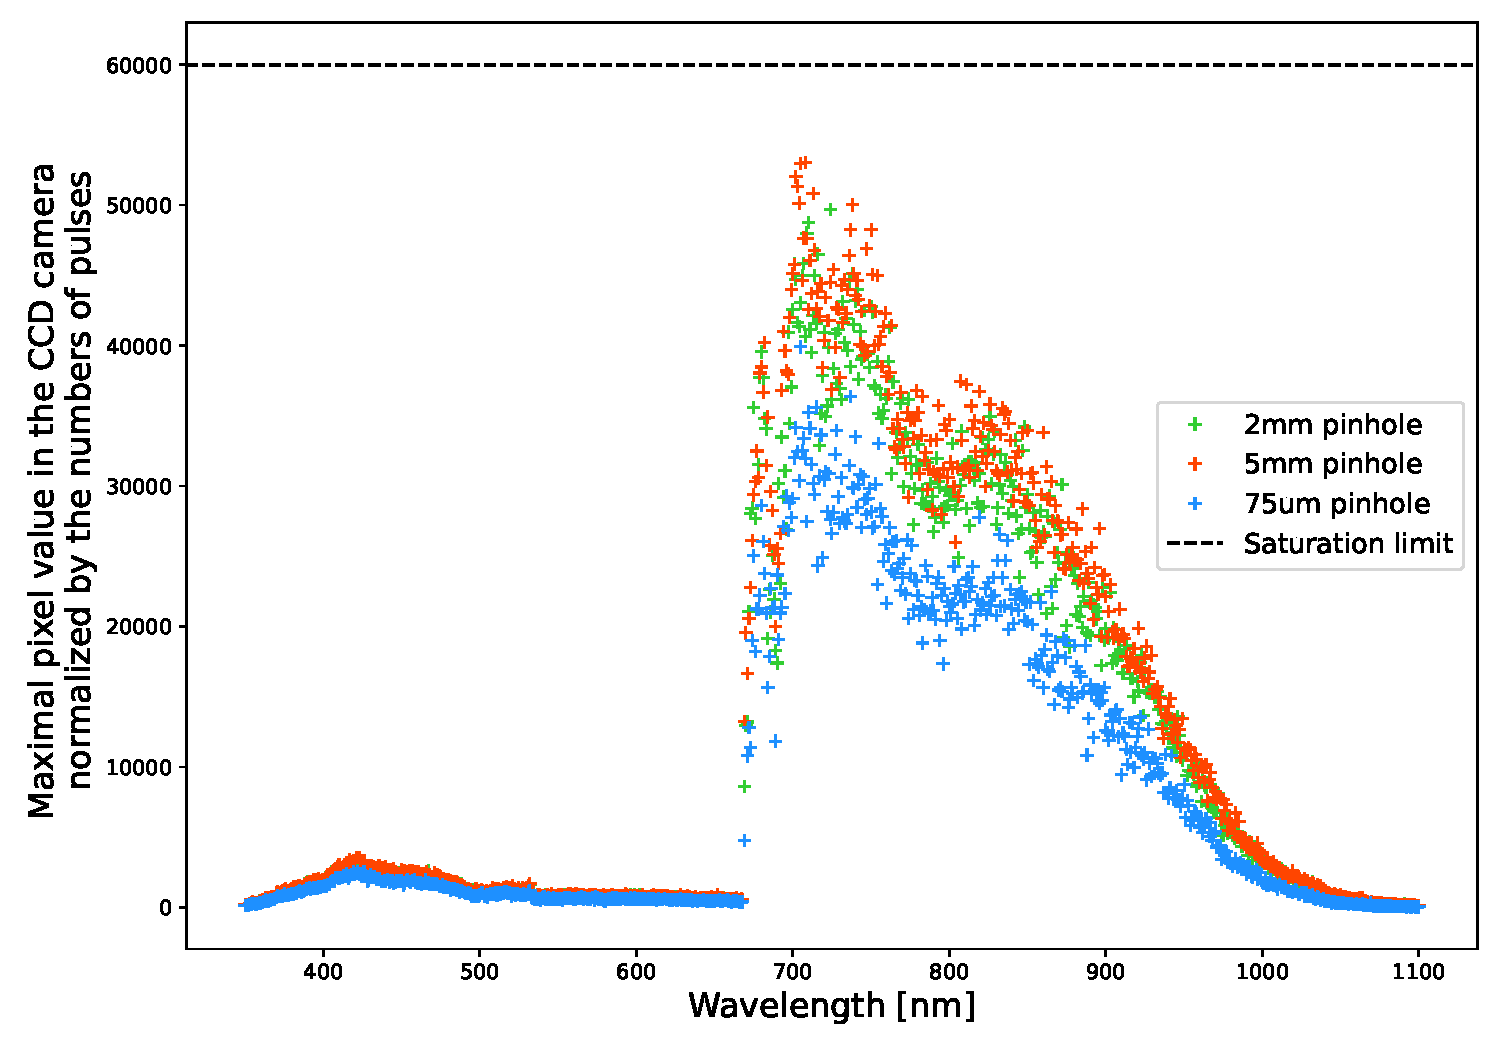
\includegraphics[width=\columnwidth]{fig/saturation_lim_ccd.pdf}
    \caption{Maximal pixel value in ADU measured in the CCD camera of \SD normalized by the number of pulses and the saturation limit of the camera estimated at \SI{61600}{ADU}, against the wavelength. Here we can see that for some wavelengths above \SI{668}{\nano\meter} a few number of pulses can saturate the camera.}
    \label{fig:saturation_lim}
    %/stardice/analysis/cbp_paper/golden_sample_analysis/dr2/npulses_stardice.ipynb
\end{figure}


\begin{itemize}
\item Images
\item Photocurrent timeseries
\item Spectral time series
\end{itemize}

\subsection{Reduction of images}
\label{sec:photometry}

In this section, the data reduction for the monitoring photodiode and the spectrograph are the same as described respectively in the section \ref{sec:pd_reduction} and \ref{sec:spectro_reduction}. Aperture photometry is done to extract the cumulated charge from the \SD camera images. This requires to estimate the background and subtract it and the background subtraction method depends on the pinhole used at the input of the CBP optics. We will described the two methods in the sections below.

\subsubsection{\spinhole pinhole}

Firstly, we load a batch of images from the same run. We compute the mean of the pixels in the overscan and subtract it to our images. We estimate $\sigma$ the standard deviation of an image, and every pixel with a signal higher than 5$\sigma$ is masked, as well as all the surrounding pixels that has a signal higher than 2$\sigma$. Then we proceed to a segmentation of the masked image into boxes of $256\times256$ pixels. We estimate the mean and the standard deviation of the background in each of these boxes, and we interpolate their values in a 2D map to get our estimation of the background. This background is subtracted to the image, then we compute the centroid of the spot of interest. We measure the number of charges $\Qccd$ with aperture photometry at a radius of 21.2 pixels (see growth curve in Figure~\ref{fig:growth_75um}).

\begin{figure}[h]
    \centering
    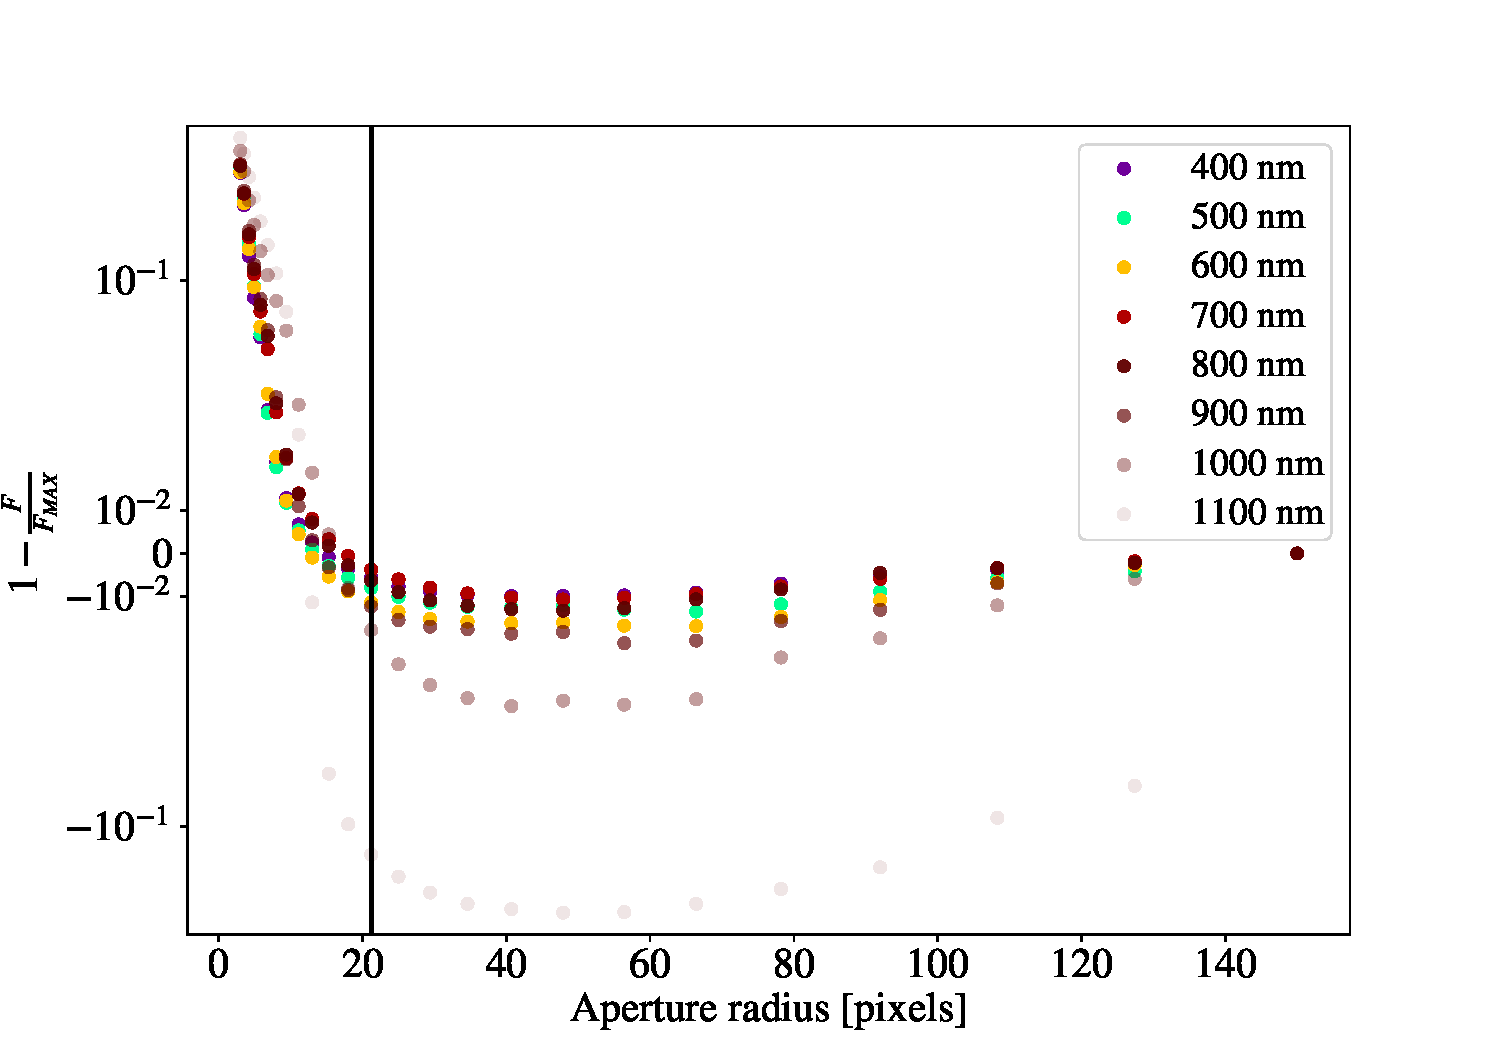
\includegraphics[width=\columnwidth]{fig/growth_curve_75um.pdf}
    \caption{Growth curve obtained with the \spinhole pinhole. Le vertical axis is obtained by computing 1 minus the flux in ADU at the radius aperture in the horizontal axis $F$, normalized by the flux maximal at the maximal aperture $F_{MAX}$. Here the maximal aperture corresponds to a radius of 56.4 pixels. The scale is linear under 0.05, and logarithmic above.}
    \label{fig:growth_75um}
    %/stardice/analysis/cbp_paper/golden_sample_analysis/dr2/growth_curves.ipynb
\end{figure}

\subsubsection{\bpinhole pinhole}

When using \bpinhole pinhole, the main spot take a significant area of the focal plane, meaning there is not enough background in the image to estimate it. This time we use images without any light coming from the CBP to estimate the background. Between each image taken with light coming from the CBP, we took background images by turning off the laser. These background images were stationary with respect to time and wavelength, as it can be seen respectively in Figure~\ref{fig:stationarity_time} and \ref{fig:stationarity_wl}. We compute a master background by doing the mean from all of these background images. Then we find the centroid of the spot of interest, and we measure the charges collected in the \SD camera by aperture photometry. We evaluate the optimal radius at 300 pixels for the \bpinhole pinhole in order to contain the main spot and the ghost (see growth curve \ref{fig:growth_5mm}). We estimate the background by doing the aperture photometry at the same position and same radius of the master background, and then subtract it to the charge measured. Finally, we can extract the charges $\Qccd$ collected in the \SD camera coming from the CBP. The same method is applied for the \SI{2}{\milli\meter} pinhole, with an aperture of 150 pixels.

\begin{figure}[h]
    \centering
    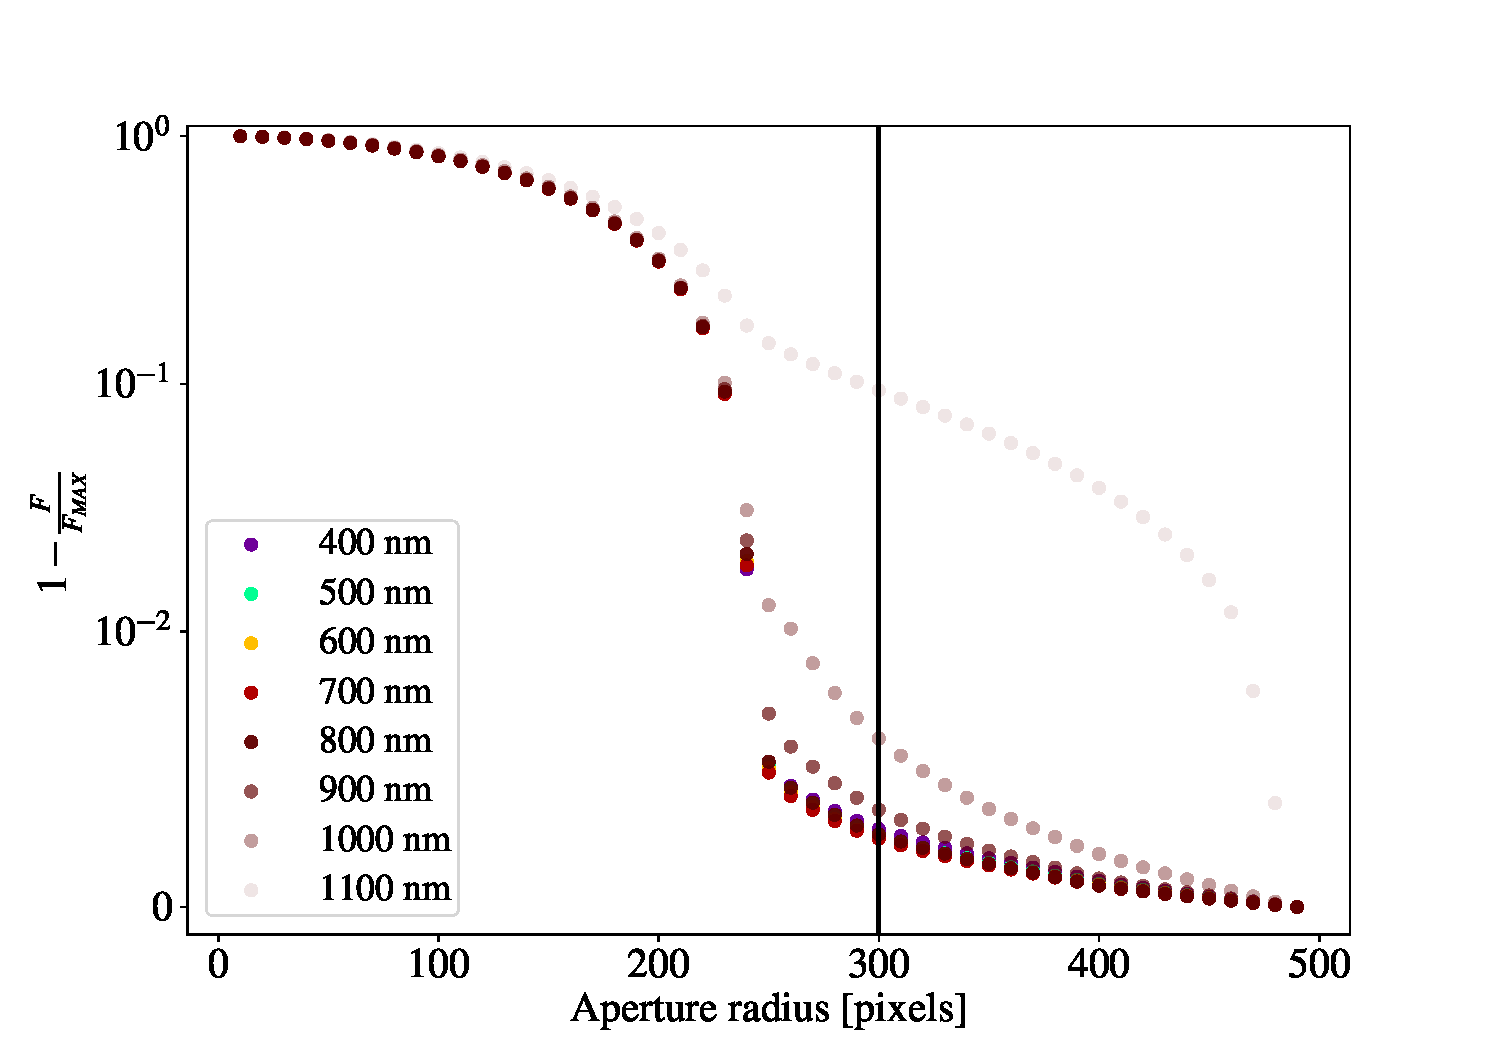
\includegraphics[width=\columnwidth]{fig/growth_curve_5mm.pdf}
    \caption{Growth curve obtained with the \spinhole pinhole. Le vertical axis is obtained by computing 1 minus the flux in ADU at the radius aperture in the horizontal axis $F$, normalized by the flux maximal at the maximal aperture $F_{MAX}$. Here the maximal aperture corresponds to a radius of 490 pixels. The scale is linear under 0.01, and logarithmic above.}
    \label{fig:growth_5mm}    
    %/stardice/analysis/cbp_paper/golden_sample_analysis/dr2/growth_curves.ipynb
\end{figure}

\com{Courbe de croissance -> problème dans l'IR : autres représentations ? ; 300 pixels contient le ghost}

\begin{figure}[h]
    \centering
    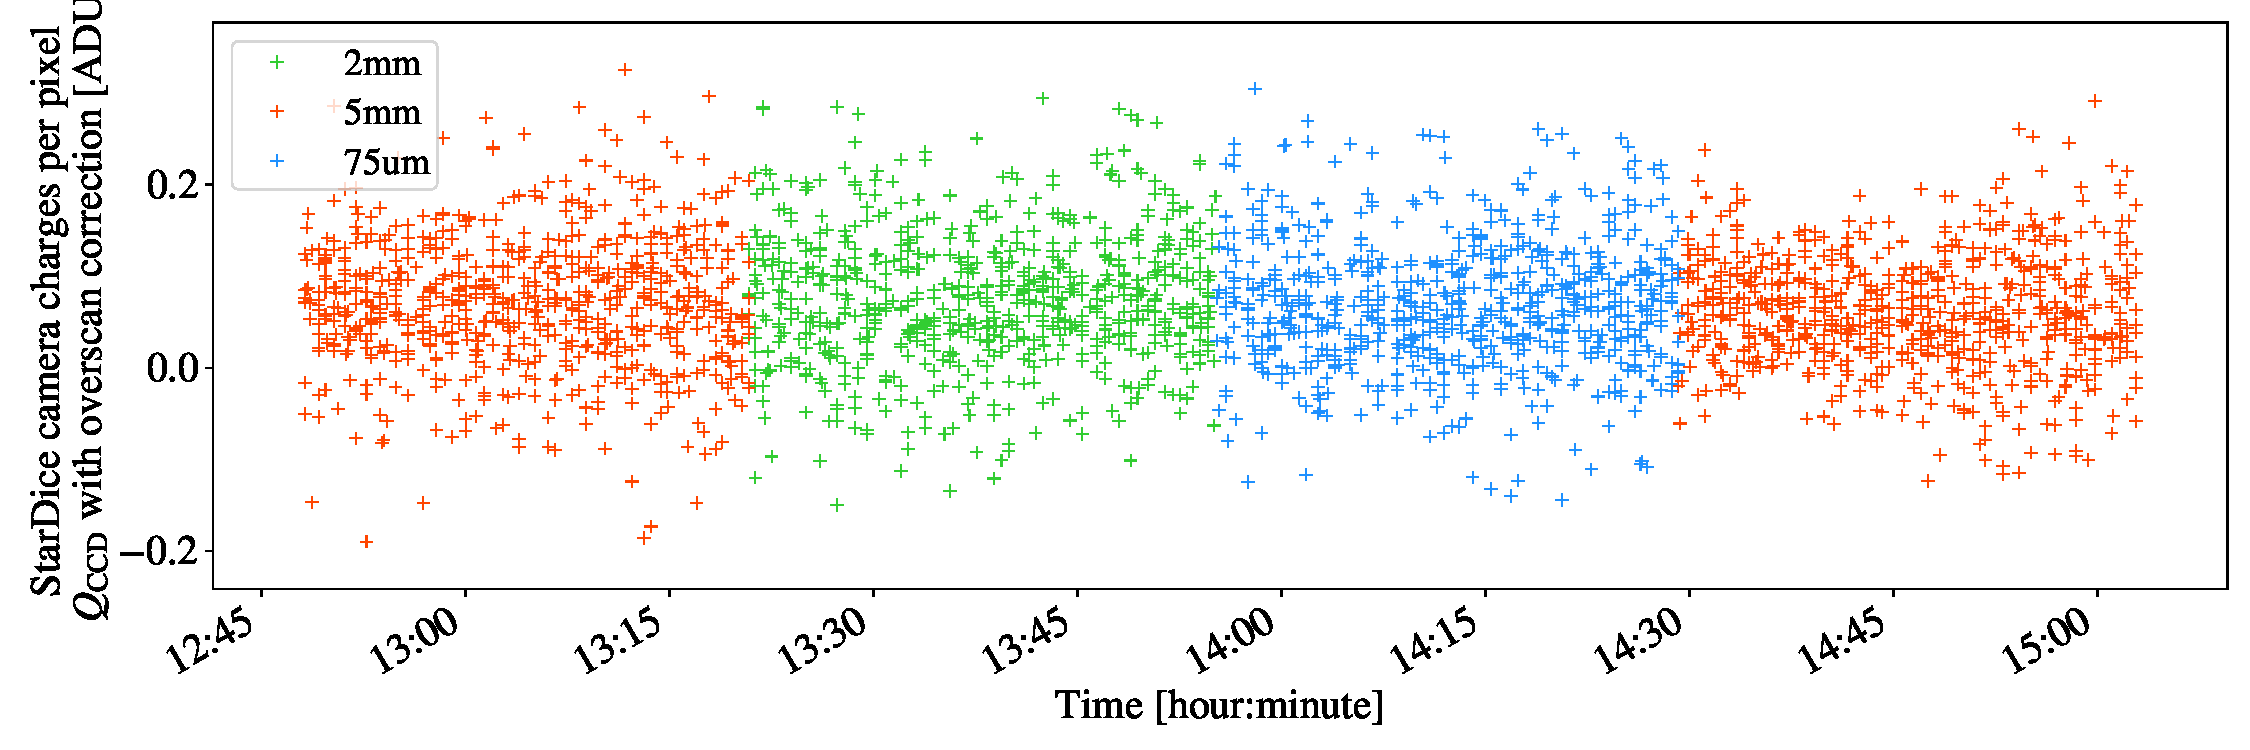
\includegraphics[width=\columnwidth]{fig/background_stationary_time.pdf}
    \caption{Charge per pixel for each background image in \SD with overscan correction with respect to the time.}
    \label{fig:stationarity_time}
    %/stardice/analysis/cbp_paper/golden_sample_analysis/dr2/background_and_centroid_stationarity.ipynb
\end{figure}

\begin{figure}[h]
    \centering
    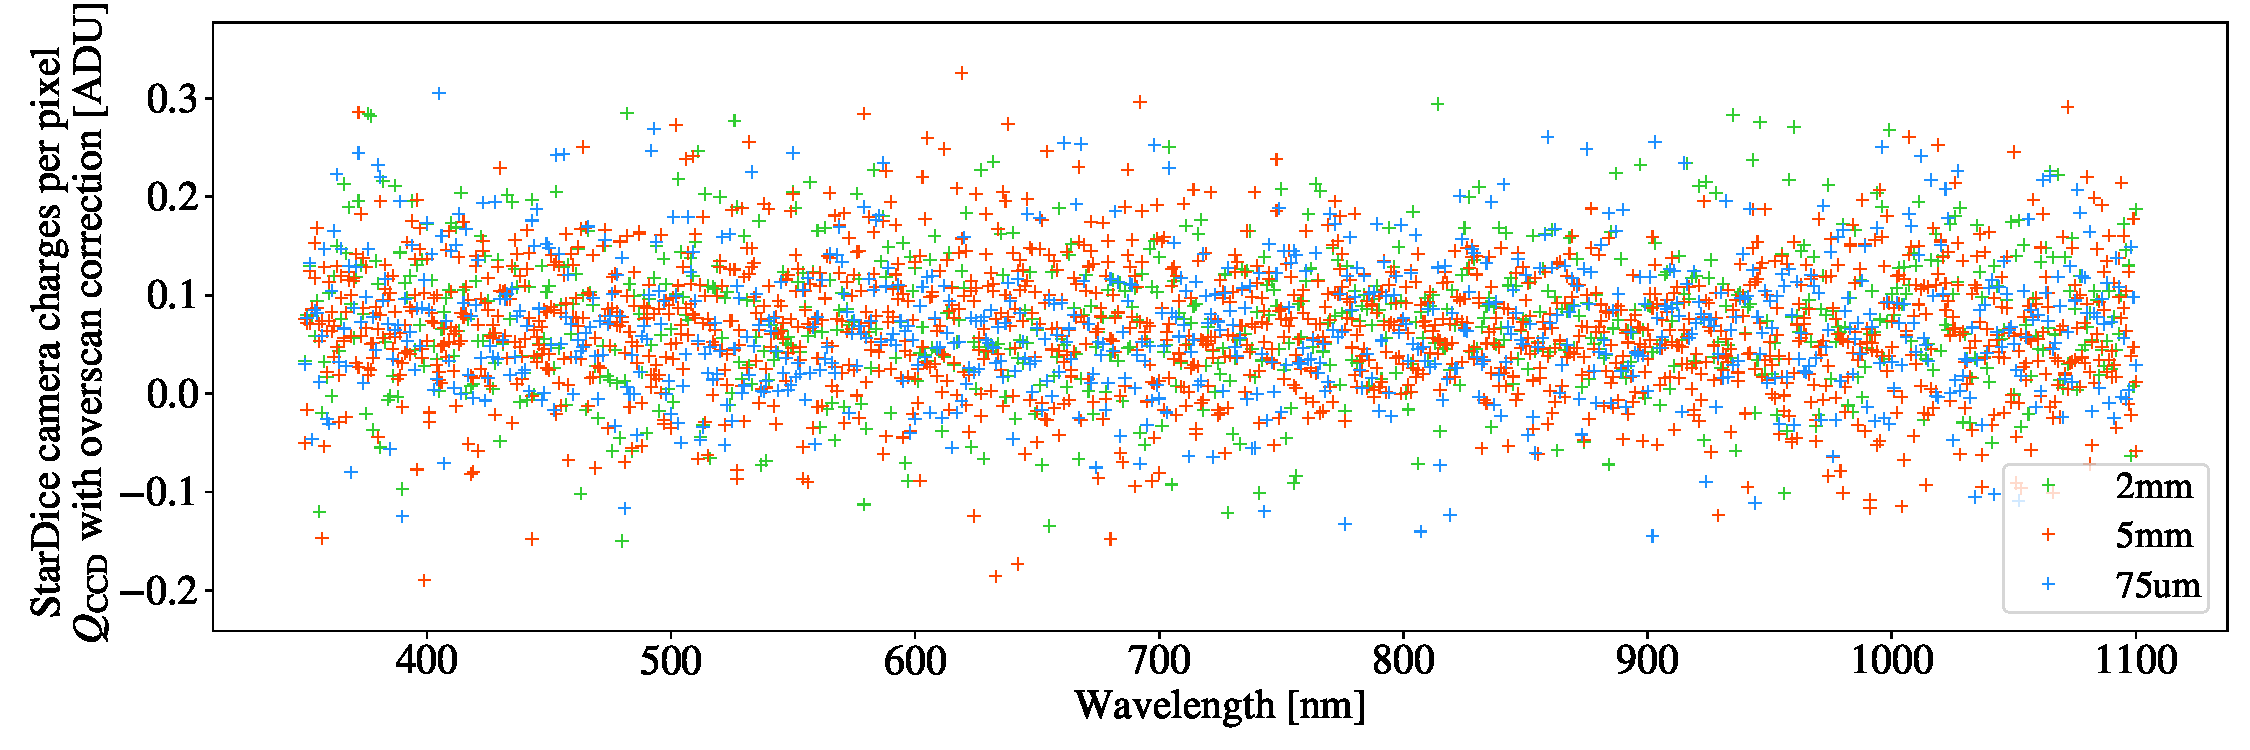
\includegraphics[width=\columnwidth]{fig/background_stationary_wavelength.pdf}
    \caption{Charge per pixel for each background image in \SD with overscan correction with respect to the wavelength.}
    \label{fig:stationarity_wl}
\end{figure}

\subsection{Correction of the \SI{532}{\nano\meter} contamination}

When extracting the charges $\Qccd$, we have to deal with the laser contamination explained in the section \ref{sec:532_cont}. The goal is to build a model for the \SI{532}{\nano\meter} contribution observed in the range [532 - 644] nm. As the photodiode and the solar cell, the total charge measured in the \SD camera $\Qccd$ is the sum of the charges from the main wavelength line $\Qccd^{\lambda_L}$ and the charges from the \SI{532}{\nm} contamination $\Qccd^{532}$. This statement cooresponds to the Equation~\ref{eq:qccd_mes}. Again, the charge measured in the photodiode $\Qphot$ is defined by the Equation~\ref{eq:qphot_mes}.
 
\begin{equation}
    \Qccd = \Qccd^{\lambda_L} + \Qccd^{532}
    \label{eq:qccd_mes}
\end{equation}

As we defined the final calibrated amount of charges detected in the photodiode per laser burst $\Qphot^{\rm cal}$, we want to do the same with the \SD CCD. The light detected by the \SD CCD has gone through the CBP optics and the \SD telescope. These instruments have respectively an optical response defined as $\Rcbp(\lambda)$ and $\Rtel(\lambda)$. We can define $R(\lambda)$ the total response of the CBP and the \SD telescope optics as in Equation~\ref{eq:rtot}. 

\begin{equation}
    R(\lambda) = \Rtel(\lambda) \times \Rcbp(\lambda)
    \label{eq:rtot}
\end{equation}

The charges $\Qccd$ can be expressed as a function of $\Rcbp$, $\Rtel$ and $\Qphot$, as shown in Equation~\ref{eq:qccd}. 

\begin{equation}
    \Qccd(\lambda) = R(\lambda) \times \Qphot(\lambda)
    \label{eq:qccd}
\end{equation}

We can compute the response $R(\lambda=532)$ can be computed thanks to the Equation~\ref{eq:rsd} because $\lambda_L = \lambda_\mathrm{comp} = 532$ nm, so all the charges detected are at the main wavelength. By combining Equations~\ref{eq:qccd_mes}, \ref{eq:qccd} and $R(\lambda=532)$, and using the $\alpha(\lambda)$ factor from \ref{eq:alpha}, we can obtain the following equation.

\begin{equation}
\begin{aligned}
    \Qccd^{\lambda_L} & = \Qccd - R(\lambda=532) \times \Qphot^{532} \\ 
    & = \Qccd - R(\lambda=532) \times \alpha(\lambda) \times \Qphot^{\lambda_L} \equiv \Qccd^{\rm cal}
    \label{eq:qccd_final}
\end{aligned}
\end{equation}

With this Equation~\ref{eq:qccd_final} we have obtained an expression for the final calibrated amount of charges detected in the \SD CCD $\Qccd^{\rm cal}$. The same can be done with the complementary wavelength line $\lambda_{\rm comp}$ appearing after $\lambda_L > \SI{1064}{\nm}$, where we use the correction coefficient $\beta$ from Equation~\ref{eq:beta} instead of $\alpha$.

\begin{figure}[h]
    \centering
    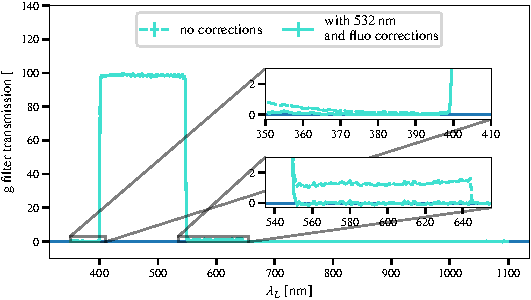
\includegraphics[width=\columnwidth]{fig/g_filter_532.pdf}
    \caption{StarDice g filter transmission as a function of the set laser wavelength $\lambda_L$, with and without the \SI{532}{\nm} correction. For clarity, we added a zoom on the out-of-band transmission where $\SI{532}{\nm}$ line is transmitted while higher wavelengths are shot by the laser.}
    \label{fig:g_filter_532}
    %cbp_paper_plots.ipynb
\end{figure}

\subsection{Intercalibration of the \SI{75}{\micro\meter} and \SI{5}{\mm} pinholes}

In Section~\ref{sec:strategy} we said that there is a need to change the pinhole in the CBP slides according to the measurement we want to do, as refered in Table~\ref{tab:schedule}. We need to ensure that we understand how the CBP response has changed when we switched the pinhole. We took measurements with the \SD telescope with both \bpinhole pinhole and \spinhole pinhole in order to intercalibrate the two pinholes, and evaluate the systematic related to this change of pinhole diameter. One major difference between the \spinhole pinhole and the \bpinhole pinhole is how the ghost and the main spot will superimpose on the focal plane.  We show in Figure~\ref{fig:schema_ghost} the optical path that produces the 1\up{st} order ghost on the focal plane. In Figure~\ref{fig:ghost_contrast}, we can see an image of the 1\up{st} order ghost next to the main spot obtained with the \spinhole pinhole. The distance between the centroïd of the main spot and the centroïd of the 1\up{st} order ghost is between 30 to 70 pixels depending on the radial position on the mirror. In the mean time, the \bpinhole pinhole photometry is made with an aperture of 300 pixels, containing the 1\up{st} order ghost and the main spot. 

\subsubsection{First order ghost photometry}

 We want to do the photometry of the 1\up{st} order ghost with the \spinhole pinhole to estimate the contribution of the ghost when we do the photometry for the \bpinhole pinhole. We build a mask with the expected ghost shape, and we fit its best position on the image. The signal measure from the 1\up{st} order ghost is simply the sum of the ADUs contained in this mask, after background subtraction. To estimate and subtract the background, we make the hypothesis that the main spot has a vertical symmetry, so we expect the background to be the same at the right and the left side of a vertical line fixed at the main spot coordinates. We place a second mask at the symmetric position from this axis of symmetry, and we measure the charges at this position, which correspond to background only. This background measurement is then subtract from the ghost photometry. The main spot emasurement is made by aperture photometry as explained in Section~\ref{sec:photometry}. 
 
 Let be $G_0$ the quantity of light collected in the main spot, and $G_\mathrm{n}$ the quantity of light collected in the ghost of order $n$. We define $\Kghost(\lambda)$ the ratio of the 1\up{st} order ghost $G_1$ over the main spot $G_0$ shown in Equation~\ref{eq:ratio_ghost}. We show this ratio measured for 5 different measurements in Figure~\ref{fig:ghost_ratio}.

\begin{equation}
    \Kghost(\lambda) = \frac{G_1(\lambda)}{G_0(\lambda)}
    \label{eq:ratio_ghost}
\end{equation}

\begin{figure}[h]
    \centering
    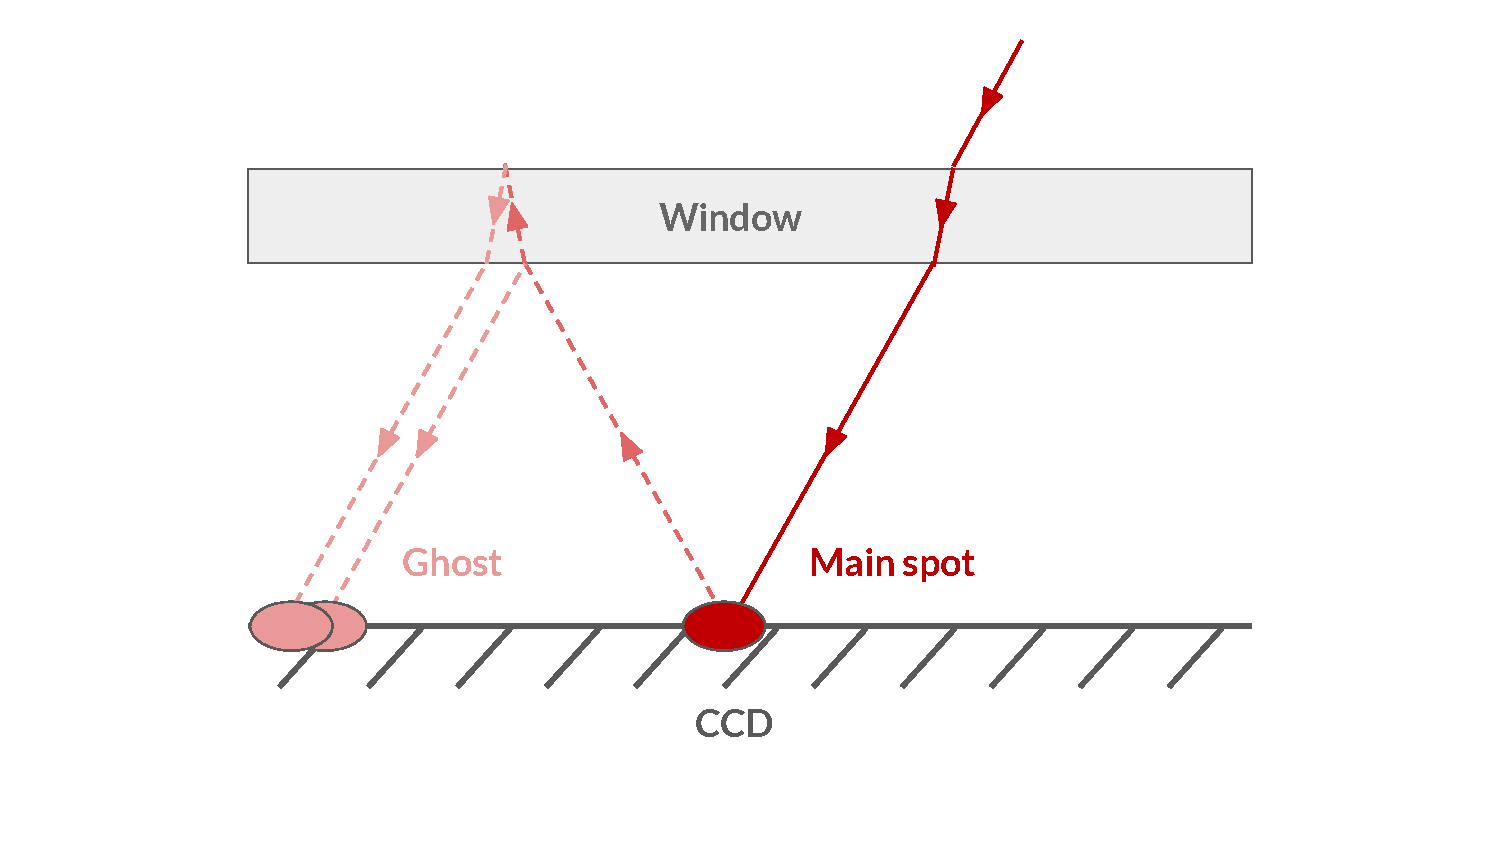
\includegraphics[width=\columnwidth]{fig/schema_ghost.pdf}
    \caption{Schematic of the origin of the ghost. A portion of the incident light reflects on the surface of the CCD, and then reflects again on one of the two faces of the window, and are then absorbed by the CCD. This creates a defocused and less intense image at an other position in the focal plane. Everytime light is absorbed by the CCD, a portion is reflected and generate a new ghost.}
    \label{fig:schema_ghost}
    %~/stardice/analysis/cbp_paper/golden_sample_analysis/dr2/ghost_photometry_general.ipynb
\end{figure}

\begin{figure}[h]
    \centering
    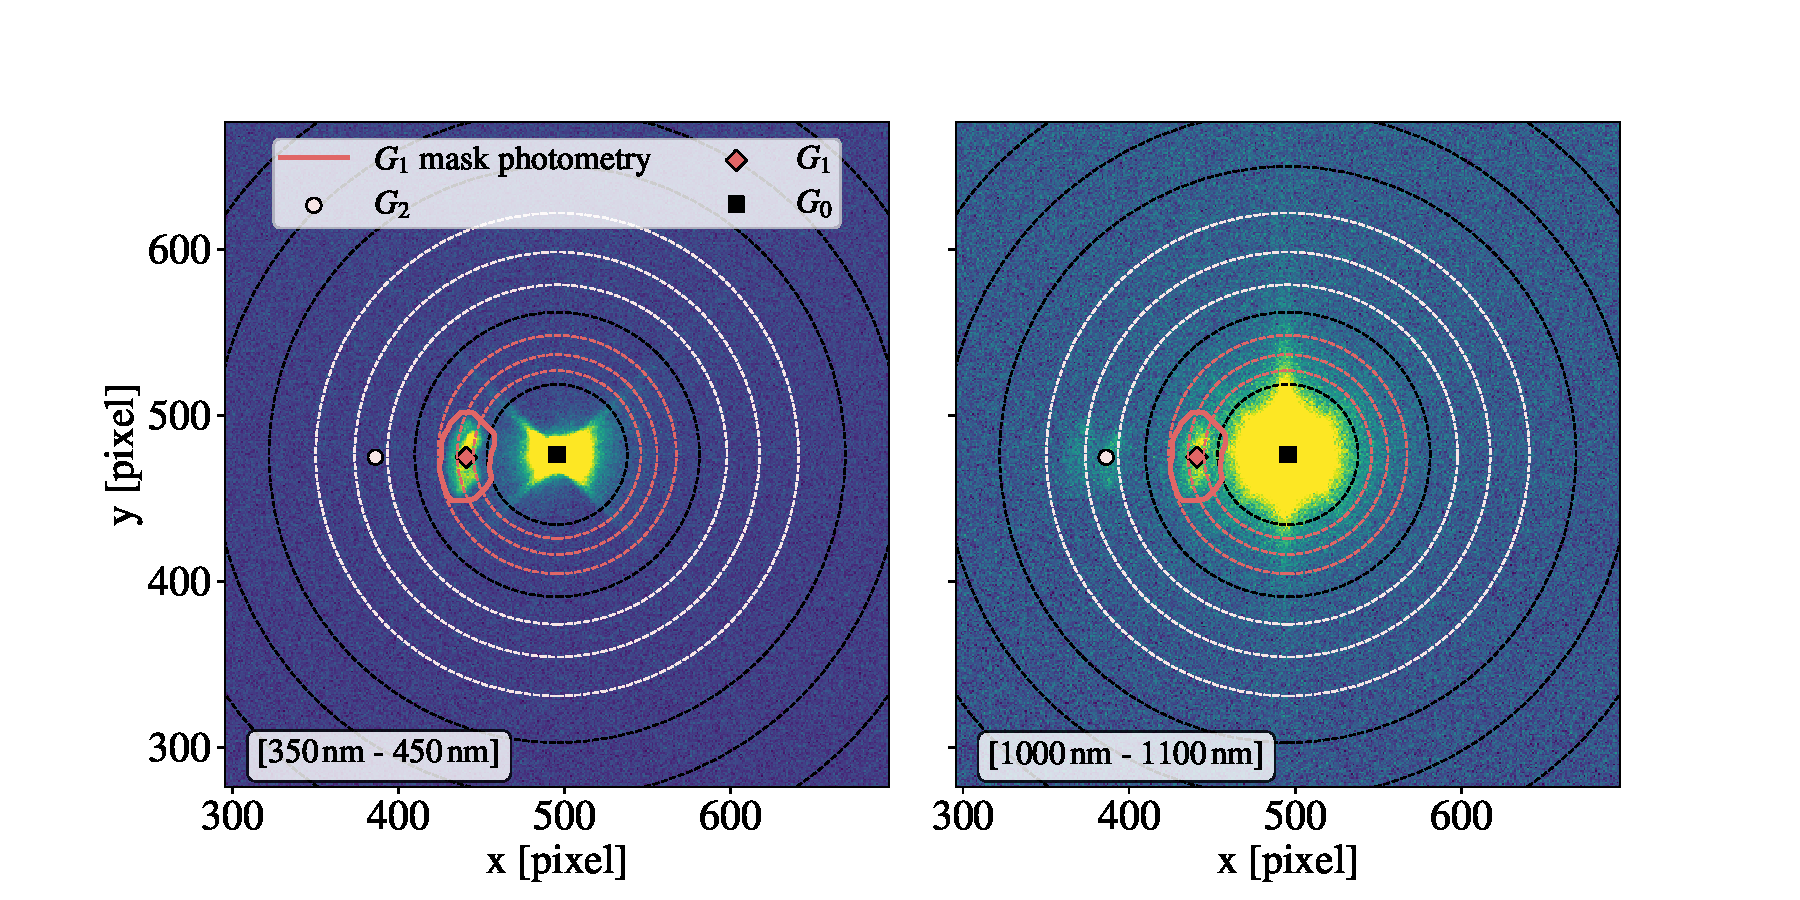
\includegraphics[width=\columnwidth]{fig/ghost_contrast.pdf}
    \caption{Image of the main spot in the center and the first order ghost at its left. The level max of the color bar is set low intentionally to make the ghost visible. The distance between the first order ghost and the main spot is between 30 and 70 pixels depending on the radial position of the point of impact on the \SD primary mirror.}
    \label{fig:ghost_contrast}
    %~/stardice/analysis/cbp_paper/golden_sample_analysis/dr2/ghost_photometry_general.ipynb
\end{figure}


 \begin{figure}[h]
     \centering
     \resizebox{\hsize}{!}{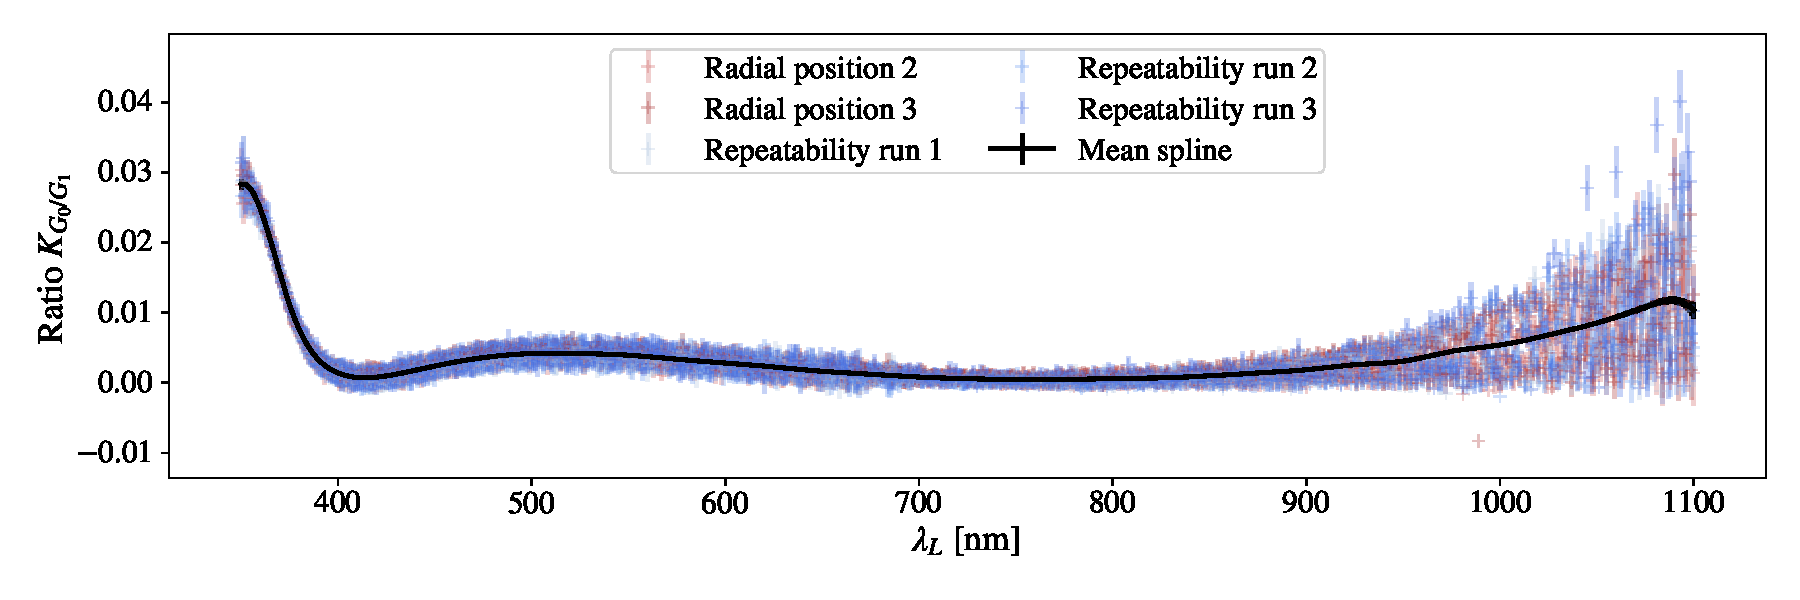
\includegraphics{fig/ghost_ratio.pdf}}
     \caption{Ratio $\Kghost$ (which correspond to the order 1 ghost $G_{1}$ over the main spot $G_0$) with respect to wavelength in nanometer. The mean spline goes through five datasets, two at different radial positions on the mirror and three at the same position. All responses are at the same position on the focal plane.}
     \label{fig:ghost_ratio}
    %~/stardice/analysis/cbp_paper/golden_sample_analysis/dr2/ghost_photometry_general.ipynb
 \end{figure}
 
 \subsubsection{Contribution of the n\up{th} order ghosts}

 Now that we did the photometry for the first order ghost, we want to study the higher orders. Since the intensity of these ghosts is very weak and hard to analyse, we will simulate their contribution from the $1^{\mathrm{st}}$ order ghost analysis. Let be $\Rwindow$ the reflection coefficient at the interface air-window and window-air, and $\Rccd$ the reflection coefficient at the interface air-CCD. We know the transmission of the window $T_\mathrm{window}$ from manufacturer datasheets, so we can infer $\Rwindow$ with the Equation~\ref{eq:rwindow}.
 
\begin{equation}
    \Rwindow = 1 - T_\mathrm{window}
    \label{eq:rwindow}
\end{equation}

 
 We define $\phi$ the flux collected by the camera, $G_0$ the quantity of light collected in the main spot, and $G_\mathrm{n}$ the quantity of light collected in the ghost of order $n$. All these quantities are linked according to the following Equations~\ref{eq:g0} and \ref{eq:gn}. The sum of all the ghosts $G_{\mathrm{n>0}}$ is defined in the Equation~\ref{eq:sum_ghost}
 \footnote{If |q| < 1, the serie $\left( \sum_{n=0}^{m} q^n \right)_{\mathrm{m \in \mathbb{N}}}$ strictly converge and \\ $\sum_{n=0}^{\infty} q^n \equiv \lim\limits_{m \rightarrow \infty} \sum_{n=0}^{m} q^n = \frac{1}{1-q}$}. %, with $R_{\mathrm{ghost}} = [2 \Rccd \Rwindow - \Rccd \Rwindow^{2}]$.

 \begin{equation}
     G_0 = (1-\Rwindow)^{2} \times (1-\Rccd) \times \phi
     \label{eq:g0}
 \end{equation}

\begin{equation}
\begin{aligned}
    G_\mathrm{n} & = G_{0} \times [\Rccd \Rwindow + \Rccd(1-\Rwindow)\Rwindow]^{n} \\
    & = G_{0} \times [2 \Rccd \Rwindow - \Rccd \Rwindow^{2}] ^{n} \\
     \label{eq:gn}
\end{aligned}
\end{equation}

 \begin{equation}
 \begin{aligned}
     G_{n>0} & = \sum_{n=0}^{\mathrm{n} \rightarrow \infty} G_\mathrm{n} - G_0 \\
     & = G_0 \times \sum_{n=0}^{n \rightarrow \infty} \left( [2 \Rccd \Rwindow - \Rccd \Rwindow^{2}] ^{n} - G_0 \right)\\
     & = G_0 \times\left( \frac{1}{1- [2 \Rccd \Rwindow - \Rccd \Rwindow^{2}]} - 1\right)
     \label{eq:sum_ghost}
 \end{aligned}
 \end{equation}

 \begin{equation}
     G_{n>1} = G_{n>0} - G_1
     \label{eq:sum_ghost_sup_1}
 \end{equation}

As we do the photometry of the 1\up{st} order ghost $G_1$, we want to verify that the ghosts of higher orders $G_{\mathrm{n}>1}$ are negligible. Using the Equations~\ref{eq:ratio_ghost}, \ref{eq:g0} and \ref{eq:gn}, we can compute $\Rccd$ with Equation~\ref{eq:rccd}.

\begin{equation}
    \Rccd = \frac{\Kghost}{\Rwindow (2 - \Rwindow)}
    \label{eq:rccd}
\end{equation}

We measured $G_1$ with aperture photometry, and we combine equations \ref{eq:rwindow}, \ref{eq:sum_ghost}, \ref{eq:sum_ghost_sup_1}, and \ref{eq:rccd} in order to compute $G_{\mathrm{n}>1}$. We show the ratio $K_{G_{\mathrm{n}>1}/G_0}$ in Figure~\ref{fig:ratio_ginf_g0}. We see that $K_{G_{\mathrm{n}>1}/G_0}$ is always below the per mil level, so we can neglect the contribution of the ghosts at order n>1. We do the hypothesis that the behaviour of the ghost is the same for the \SI{2}{\milli\meter} pinhole.

\begin{figure}[h]
    \centering
    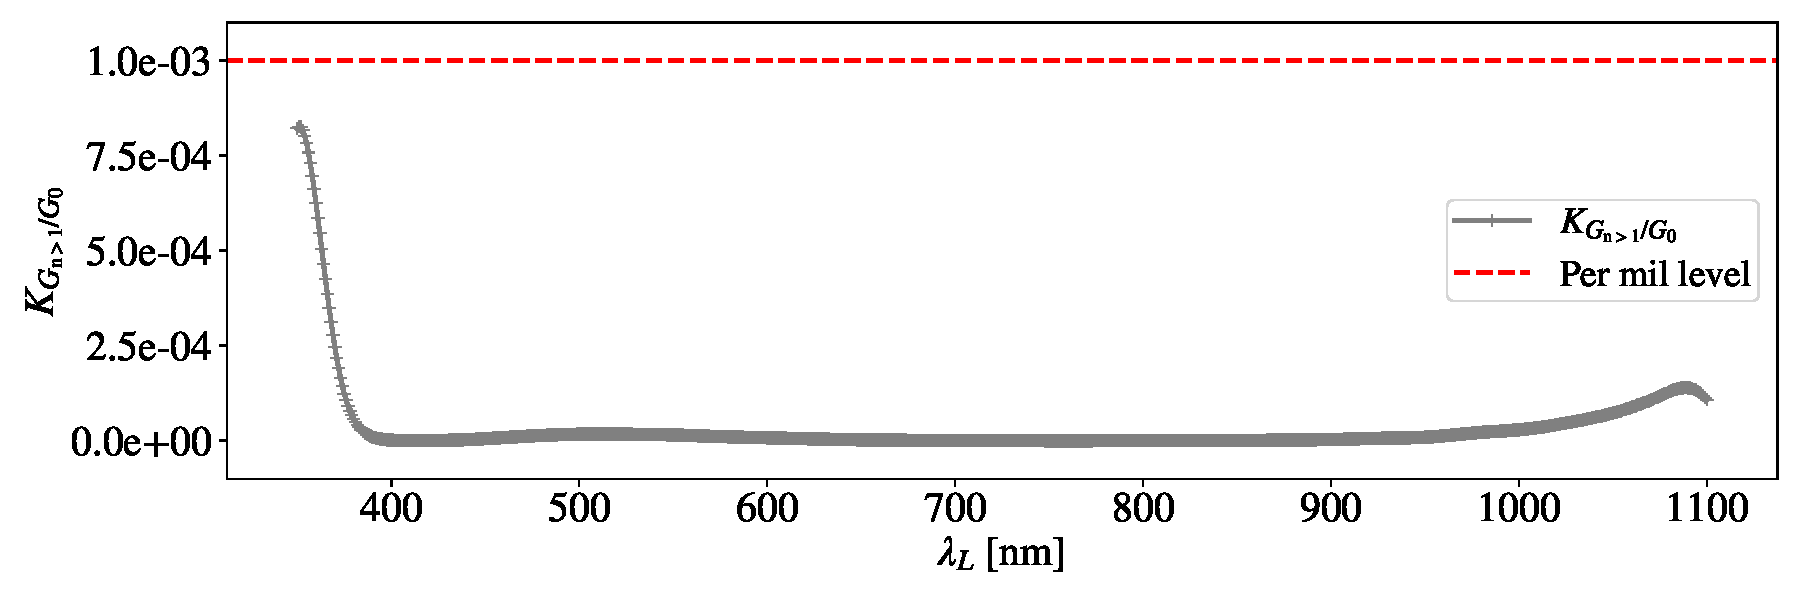
\includegraphics[width=\columnwidth]{fig/ratio_g1_ginf.pdf}
    \caption{Ratio $K_{G_{\mathrm{n}>1}/G_0}$ (which correspond to the sum of the ghosts at order higher than 1 $G_{\mathrm{n}>1}$ over the main spot $G_0$) with respect to the wavelength in nanometer.}
    \label{fig:ratio_ginf_g0}
    %~/stardice/analysis/cbp_paper/golden_sample_analysis/dr2/ghost_convergence.ipynb   
\end{figure}

\subsubsection{Ghost contribution for \bpinhole pinhole}

The total charges $\Qccd{}_{, \, \SI{5}{\milli\meter}}$ measured by doing the aperture photometry at 300 pixels for the \bpinhole pinhole is the sum of the charges $Q_0$ in the main spot $G_0$ and the charges $\Qghost$ in the 1\up{st} order ghost $G_1$. These quantities are defined by the following equations \ref{eq:qghost} and \ref{eq:qmain}, with $\Eccd$ the quantum efficiency of the StarDice CCD camera. We use the Equation~\ref{eq:ratio_ghost} to develop the Equation~\ref{eq:qccd_5mm}. Thanks to Equation~\ref{eq:qccd_5mm} we can extract $Q_0$ and study only the charges from the main spot.

\begin{equation}
    \Qghost = G_1 \times \Eccd
    \label{eq:qghost}
\end{equation}

\begin{equation}
    Q_0 = G_0 \times \Eccd
    \label{eq:qmain}
\end{equation}

\begin{equation}
\begin{aligned}
    Q_0 & = \Qccd{}_{, \, \SI{5}{\milli\meter}} - \Qghost \\
    & = \frac{\Qccd{}_{, \, \SI{5}{\milli\meter}}}{1 + \Kghost}
    \label{eq:qccd_5mm}
\end{aligned}
\end{equation}

Once we have corrected the \bpinhole pinhole from the ghost contribution, we can compute the ratio between the \SD responses defined as $\Kpinholes(\lambda)$ in Equation~\ref{eq:ratio_pinholes}. Thanks to this equation, we can infer $\Rcbp^{\spinhole}(\lambda)$ from the measurement of $\Rcbp^{\bpinhole}(\lambda)$.

\begin{equation}
    \Kpinholes(\lambda) = \frac{\Rcbp^{\bpinhole}(\lambda)}{\Rcbp^{\spinhole}(\lambda)}
    \label{eq:ratio_pinholes}
\end{equation}

We show these ratios before and after the ghost correction in the upper Figure~\ref{fig:ratio_pinholes}. We expect the ratio to be linear since it should be the ratio of two surfaces, so we draw a linear spline through the data. In the ultraviolet below \SI{400}{\nm} where the window is highly reflective, we see that the ghost correction has flattened the ratios. Above \SI{900}{\nm} we can see a significative difference between the ratio and the linear spline. This phenomenon is not quite understood and is discussed in section \ref{sec:discussion}, but we precise that the linear fit is made only for the wavelengths below \SI{900}{\nano\meter}. 

\begin{figure}[h]
    \centering
    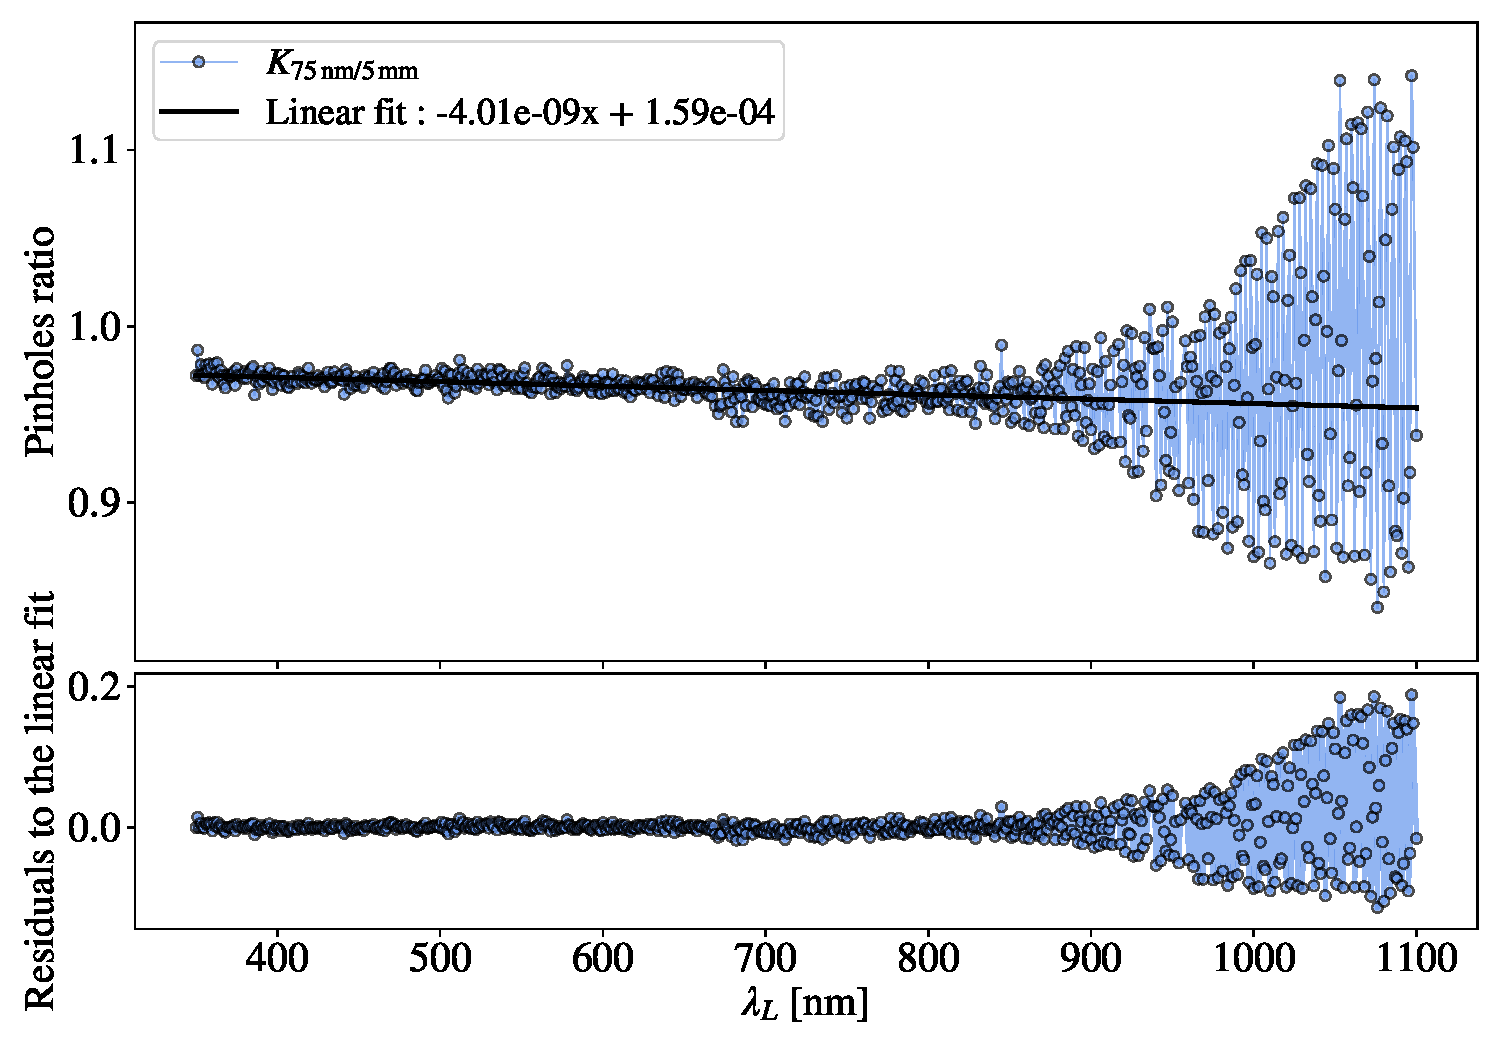
\includegraphics[width=\columnwidth]{fig/ratio_pinholes.pdf}
    \caption{Ratio $\Kpinholes(\lambda)$ with respect to wavelength, before and after ghost correction. We compute a linear spline that best fit the data between \SI{400}{\nm} and \SI{900}{\nm}.}
    \label{fig:ratio_pinholes}
    %~/stardice/analysis/cbp_paper/golden_sample_analysis/dr2/ratio_pinholes.ipynb
\end{figure}

\subsubsection{Summary}

The summary of the error budget on the \SD telescope response id detailed in Figure~\ref{fig:sd_budget}


\begin{figure}
    \centering
    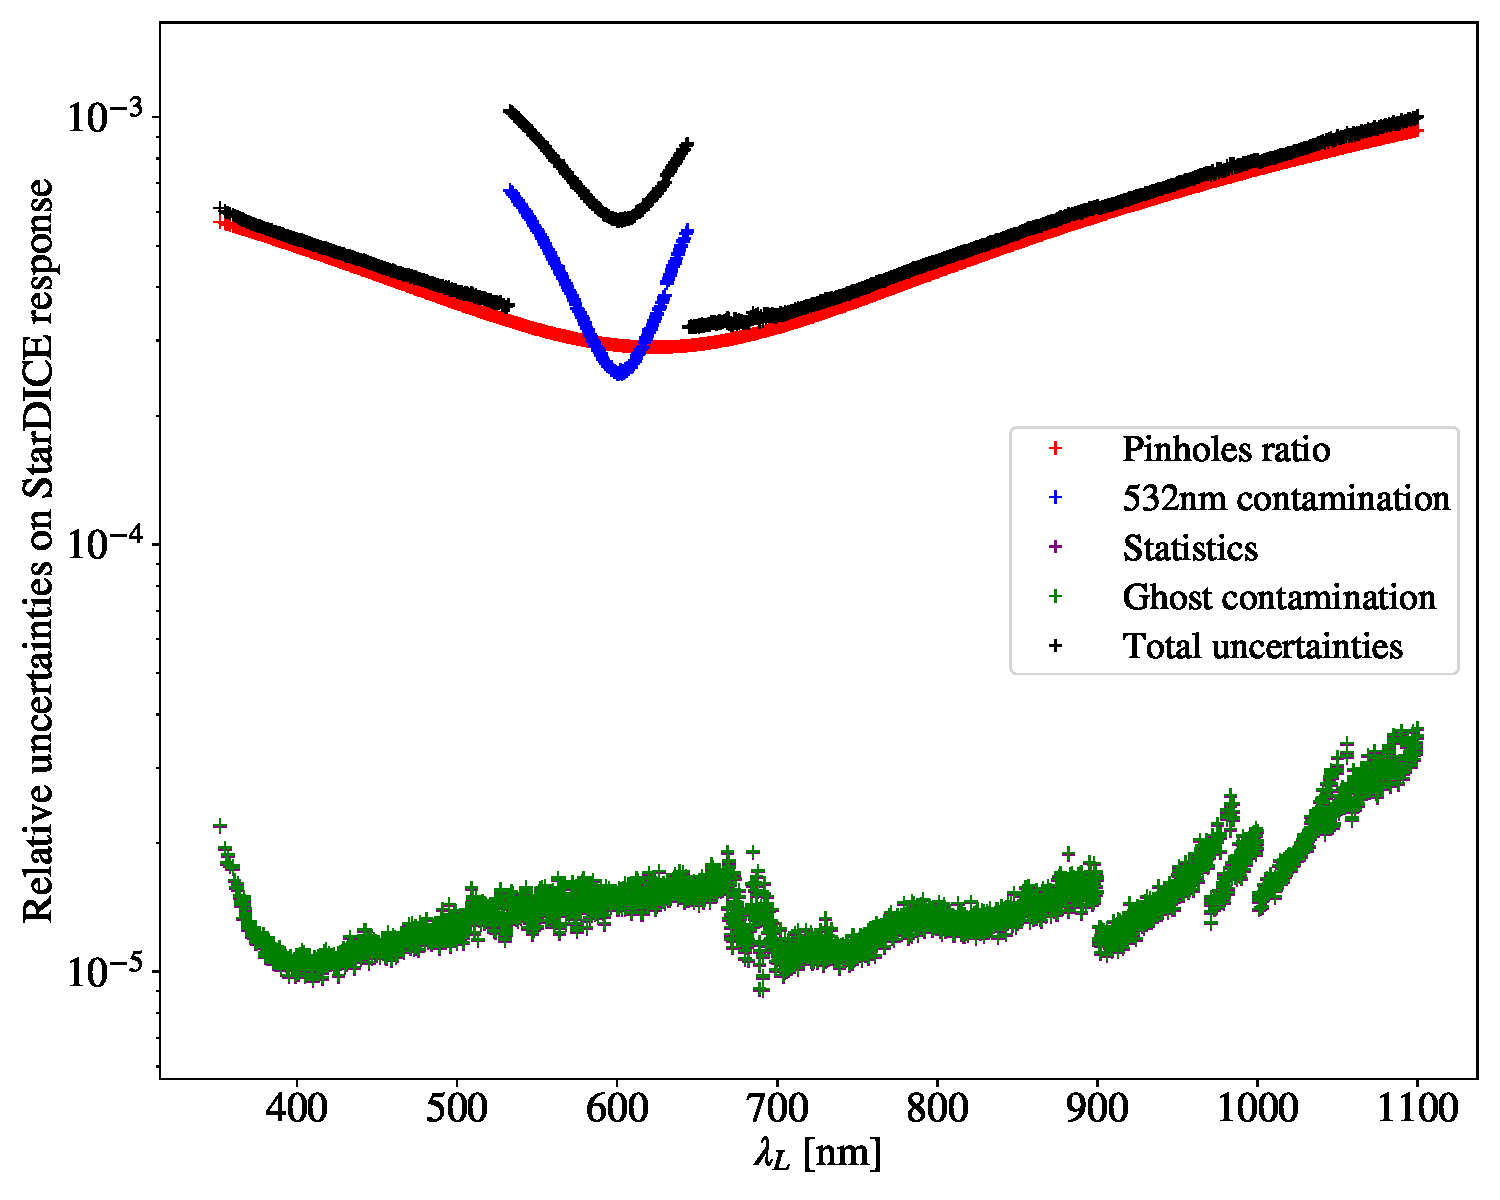
\includegraphics[width=\columnwidth]{fig/sd_uncertainties_budget.pdf}
    \caption{Total error budget for \SD response.}
    \label{fig:sd_budget}
\end{figure}

\subsection{\SD response scan}

\subsubsection{\SD optics, filters and grating responses}

In this section we will present the results of our different measurements. The following measurements are all taken at the same position on the mirror and the focal plane. The Figure~\ref{fig:stardice_5mm_response} show the \SD response obtained with the \bpinhole pinhole, and no filter. The Figure~\ref{fig:stardice_75um_response} show the \SD response obtained with the \spinhole pinhole, with all filters. In this figure we have a wavelength resolution sufficient enough to see the filter edges. The Figure~\ref{fig:stardice_grating_response} show the \SD response obtained with the \spinhole pinhole, with the grating set in front of the camera. The grating being blazed so that the 1\up{st} order of diffraction is the brightest, so we will mainly focus on this order of diffraction. We see a cut of the 2\up{nd} and 3\up{rd} order that correspond to the wavelength at which the signal is outside the CCD sensor.

\begin{figure}[h]
    \centering
    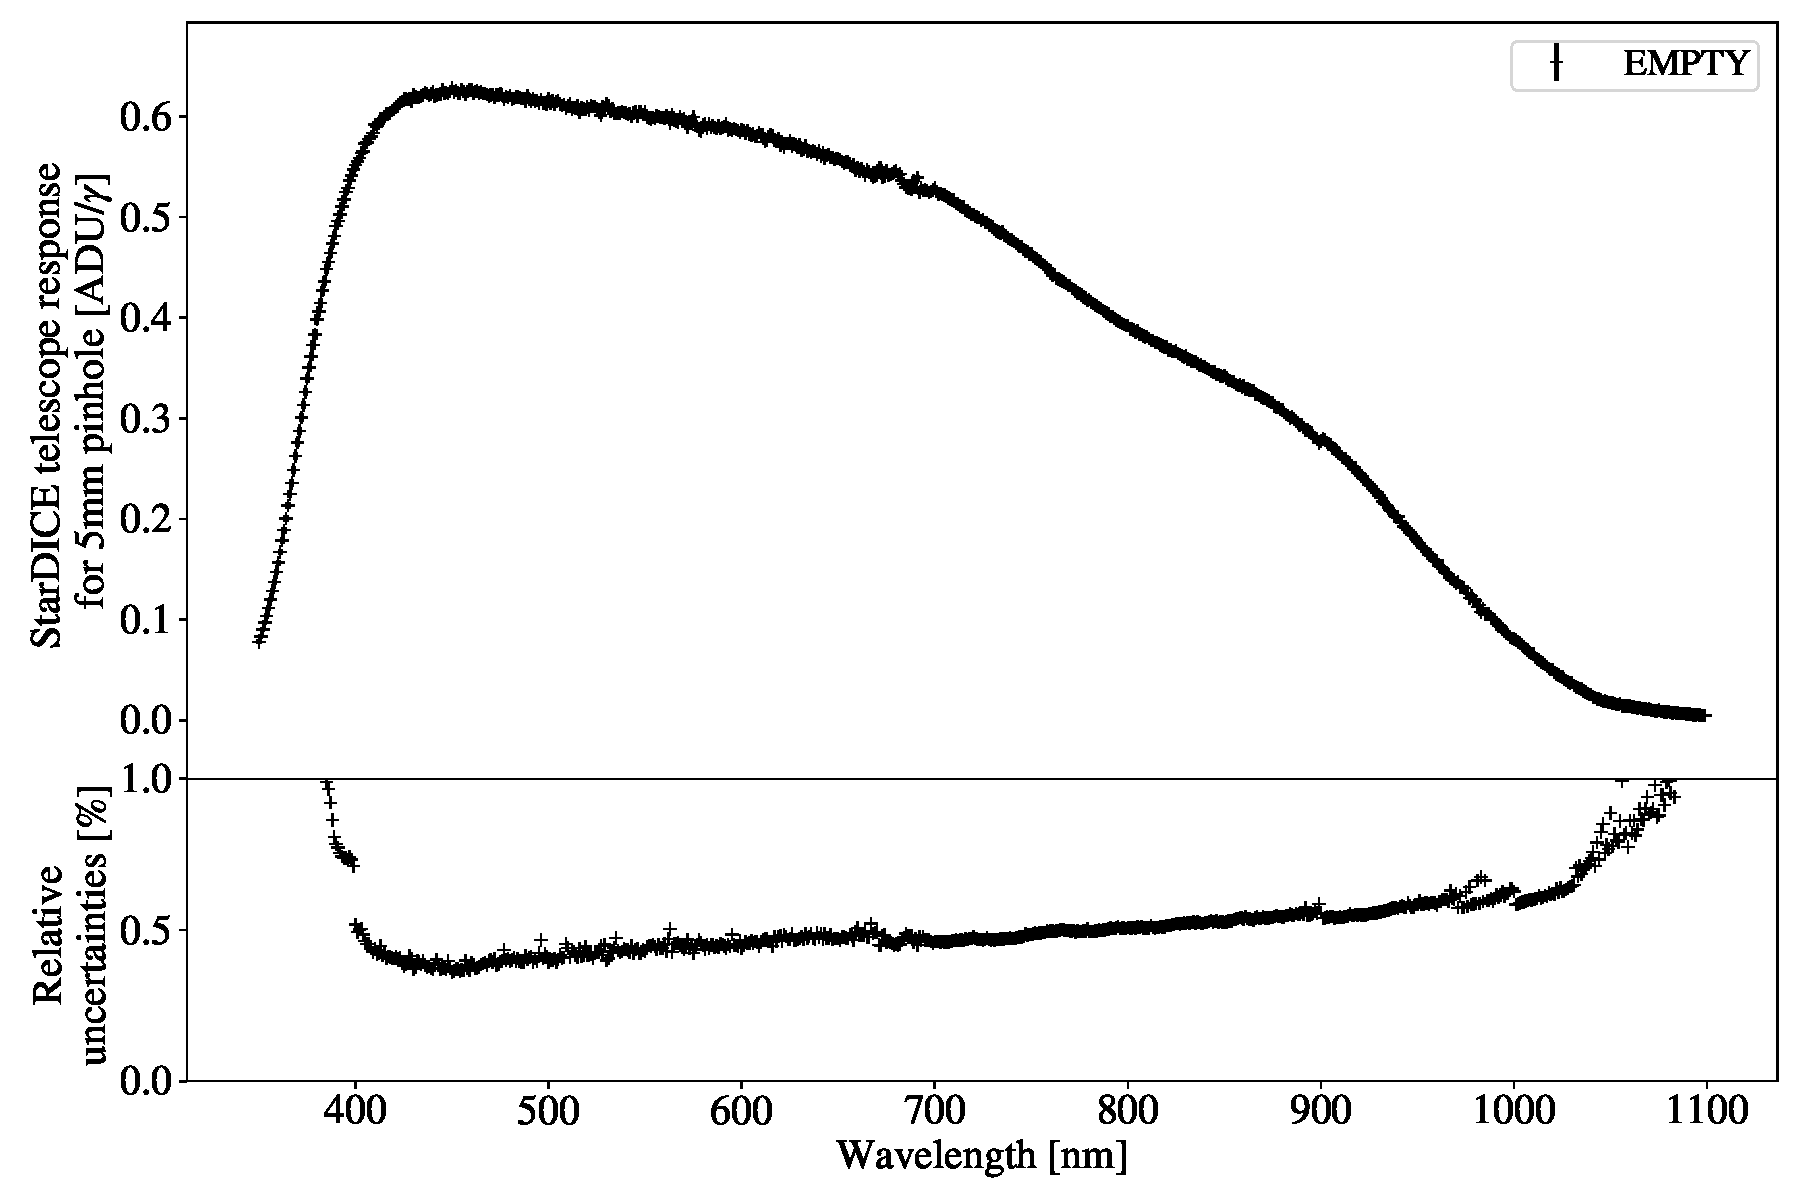
\includegraphics[width=\columnwidth]{fig/stardice_5mm_response.pdf}
    \caption{Up : \SD response with no filter and \bpinhole pinhole with respect to wavelength in nanometer. Bottom : Uncertainties over the \SD response measurement with respect to wavelength in nanometer.}
    \label{fig:stardice_5mm_response}
    %~/stardice/analysis/cbp_paper/golden_sample_analysis/dr2/response_plots.ipynb
\end{figure}

\begin{figure}[h]
    \centering
    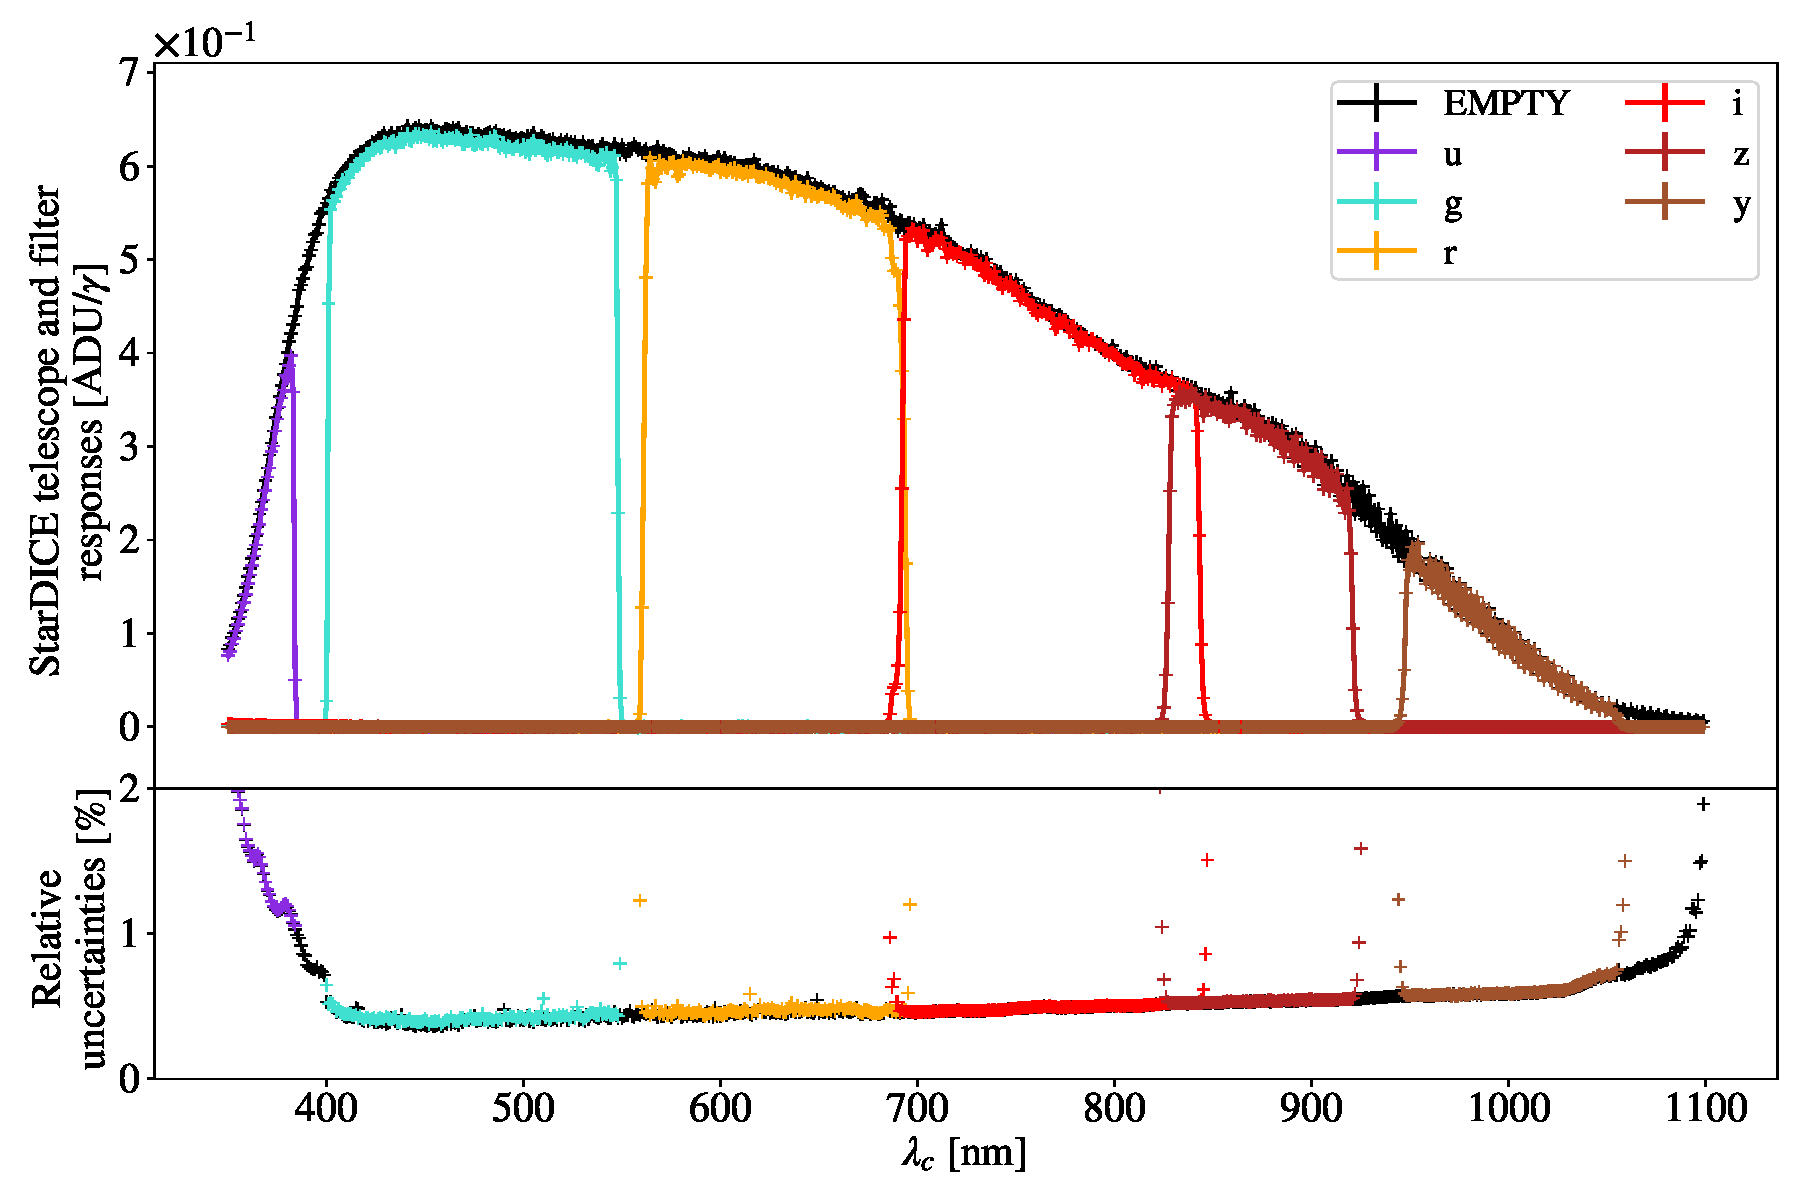
\includegraphics[width=\columnwidth]{fig/stardice_75um_response.pdf}
    \caption{Up : \SD response with at all filters and \spinhole pinhole with respect to wavelength in nanometer. Bottom : Uncertainties over the \SD response measurement with respect to wavelength in nanometer.}
    \label{fig:stardice_75um_response}
    %~/stardice/analysis/cbp_paper/golden_sample_analysis/dr2/response_plots.ipynb
\end{figure}

\begin{figure}[h]
    \centering
    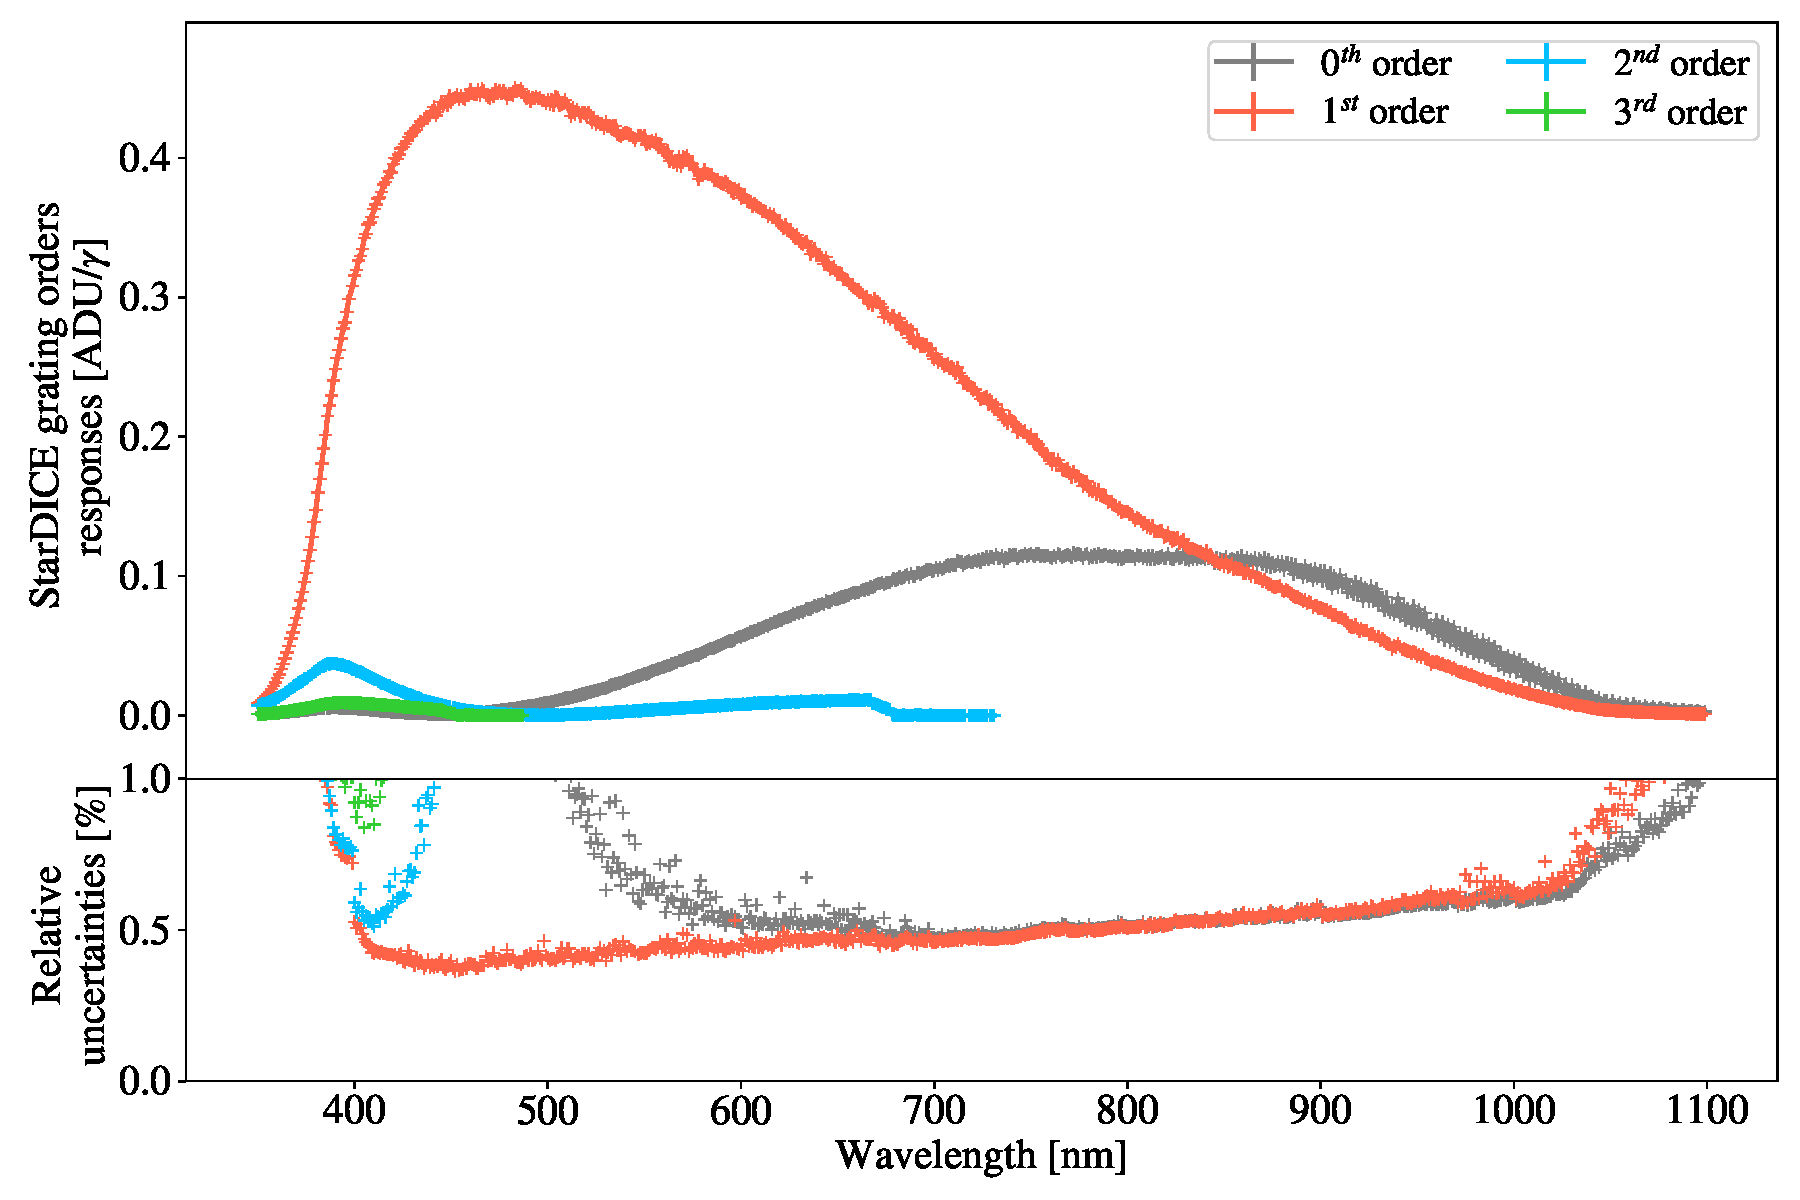
\includegraphics[width=\columnwidth]{fig/stardice_grating_response.pdf}
    \caption{Up : \SD response with the grating in front of the camera and \spinhole pinhole with respect to wavelength in nanometer. Bottom : Uncertainties over the \SD response measurement with respect to wavelength in nanometer.}
    \label{fig:stardice_grating_response}
    %~/stardice/analysis/cbp_paper/golden_sample_analysis/dr2/response_plots.ipynb
\end{figure}

\subsubsection{Radial positions}

The upper Figure~\ref{fig:radial_positions} show the \SD response obtained with the \spinhole pinhole and without filters for the different radial positions on the mirror shown in Figure~\ref{fig:8_mirror_positions} left, and the same focal plane position. The lower figure show the normalized residuals to the mean spline going through the four responses. In the ultraviolet below \SI{450}{\nm}, we can see a significant difference between the four radial positions. It goes up to 30\%, and it will be discussed in the section \ref{sec:discussion}. What we see above \SI{1000}{\nm} in the infrared is the result of the data oscillations around the spline caused by the fringing. 

\begin{figure}[h]
    \centering
    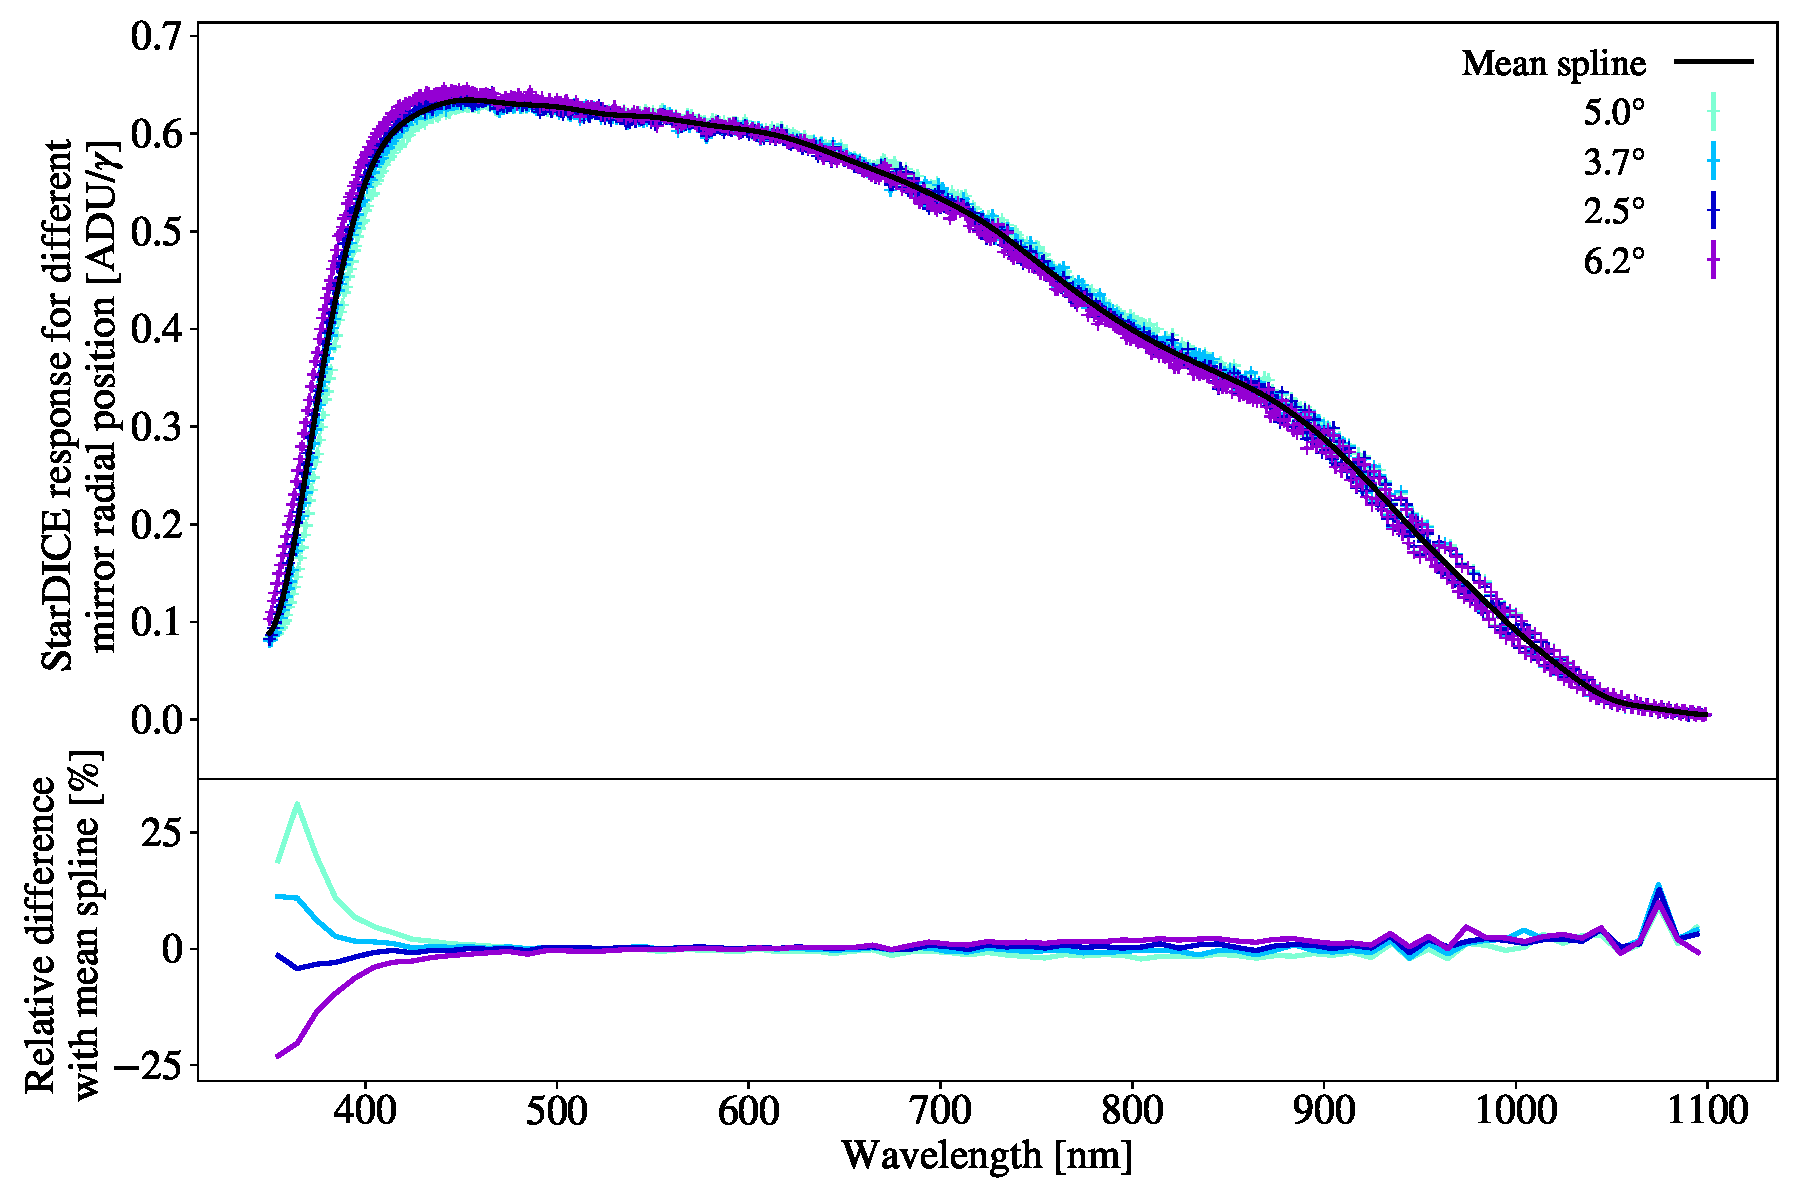
\includegraphics[width=\columnwidth]{fig/radial_positions.pdf}
    \caption{Top : \SD response for the different radial positions on the mirror, but same position on the focal plane. Bottom : Relative difference between the data and the mean spline.}
    \label{fig:radial_positions}
    %~/stardice/analysis/cbp_paper/golden_sample_analysis/dr2/2022_03_01_stardice_transmission_radius.ipynb
\end{figure}

\subsubsection{Quadrant positions}

The upper Figure~\ref{fig:radial_positions} show the \SD response obtained with the \spinhole pinhole and without filters for the different quadrant positions on the mirror shown in Figure~\ref{fig:8_mirror_positions} right, and the same focal plane position. The lower figure show the normalized residuals to the mean spline going through the four responses. We see again a divergence below \SI{400}{\nm} of about 20\% at most. The phenomenon in the infrared is still caused by the fringing. 

\begin{figure}[h]
    \centering
    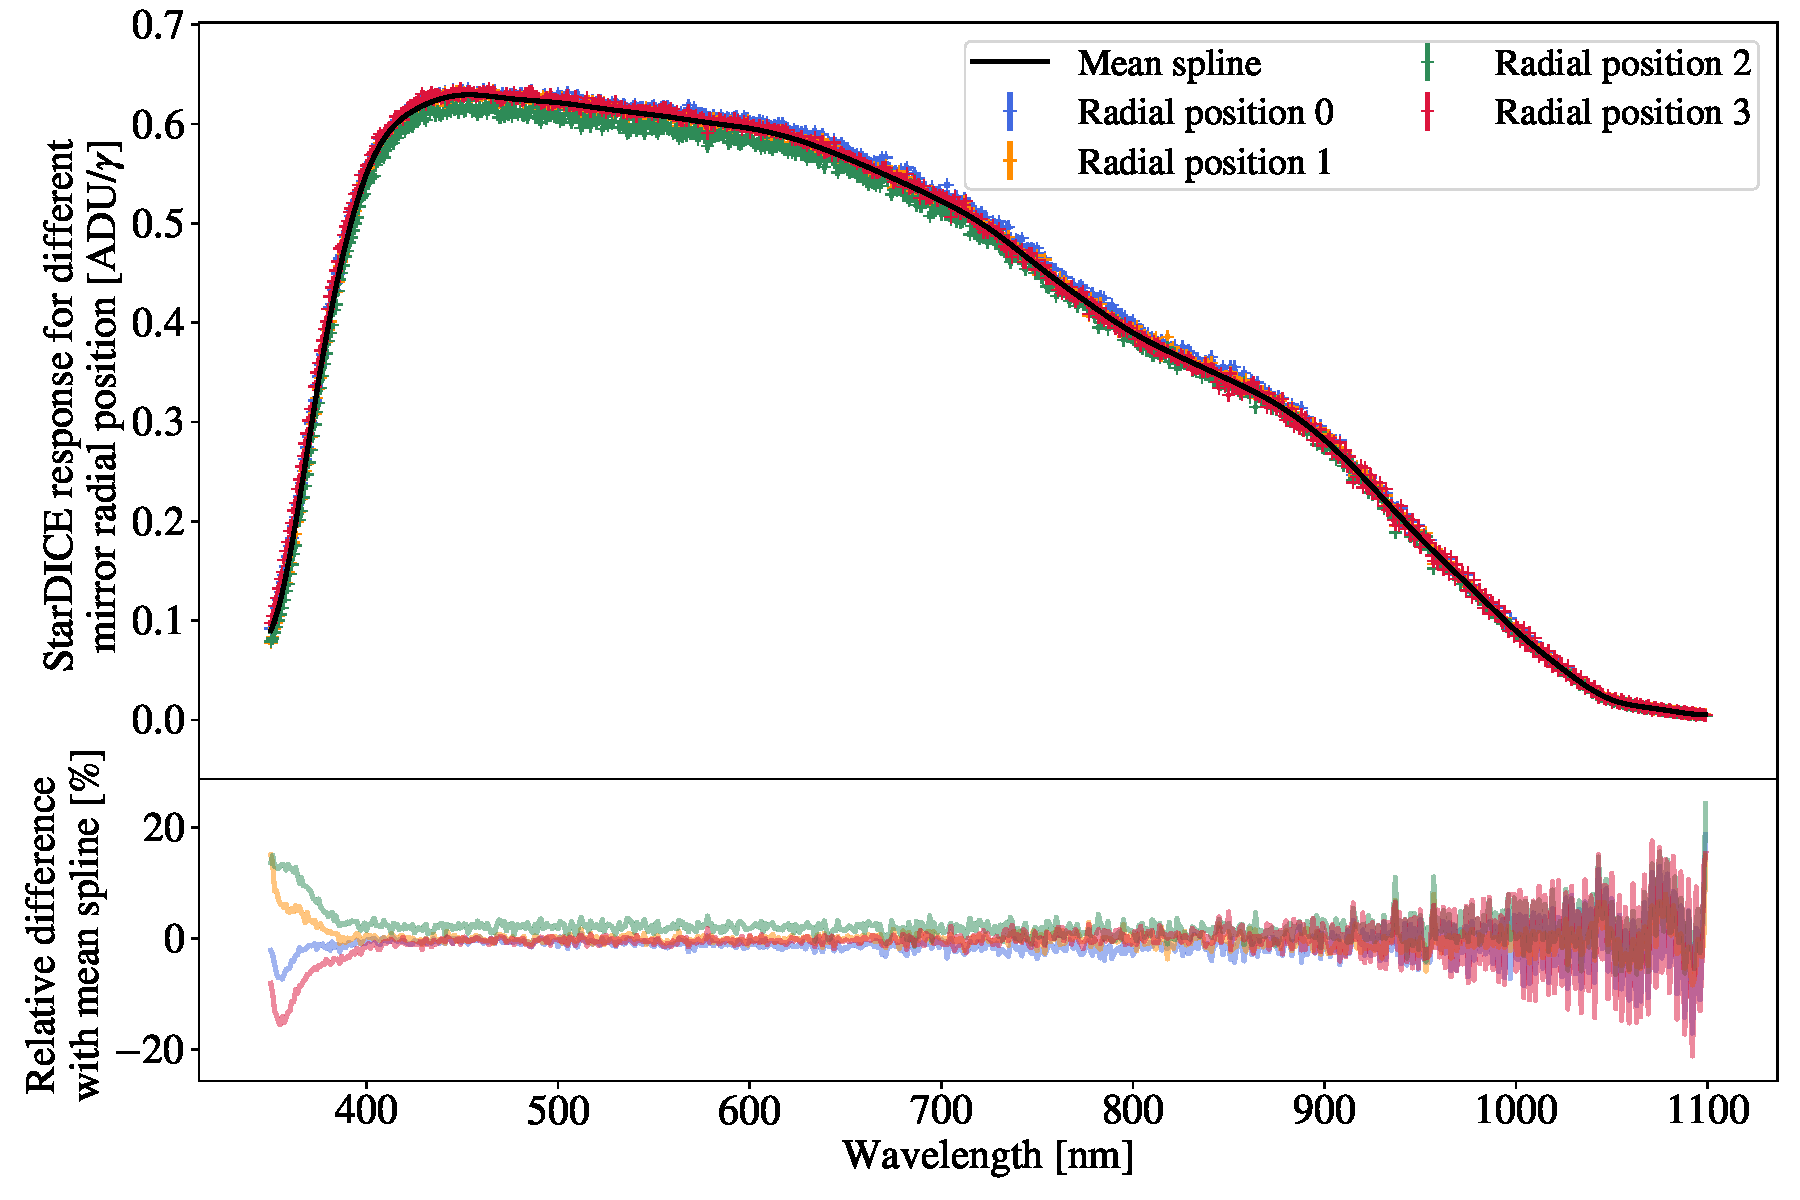
\includegraphics[width=\columnwidth]{fig/quadrant_positions.pdf}
    \caption{Top : \SD response for the different quadrant positions on the mirror, but same position on the focal plane. Bottom : Relative difference between the data and the mean spline.}
    \label{fig:quadrant_positions}
    %~/stardice/analysis/cbp_paper/golden_sample_analysis/dr2/2022_03_01_stardice_transmission_mirror_samples.ipynb
\end{figure}

\subsubsection{Focal plane positions}

The upper Figure~\ref{fig:ccd_positions} show the \SD response obtained with the \spinhole pinhole and without filters for the same radial and quadrant position on the mirror, and the different focal planes positions from the grid show in Figure~\ref{fig:ccd_grid}. The lower figure show the normalized residuals to the mean spline going through the sixteen responses.

\begin{figure}[h]
    \centering
    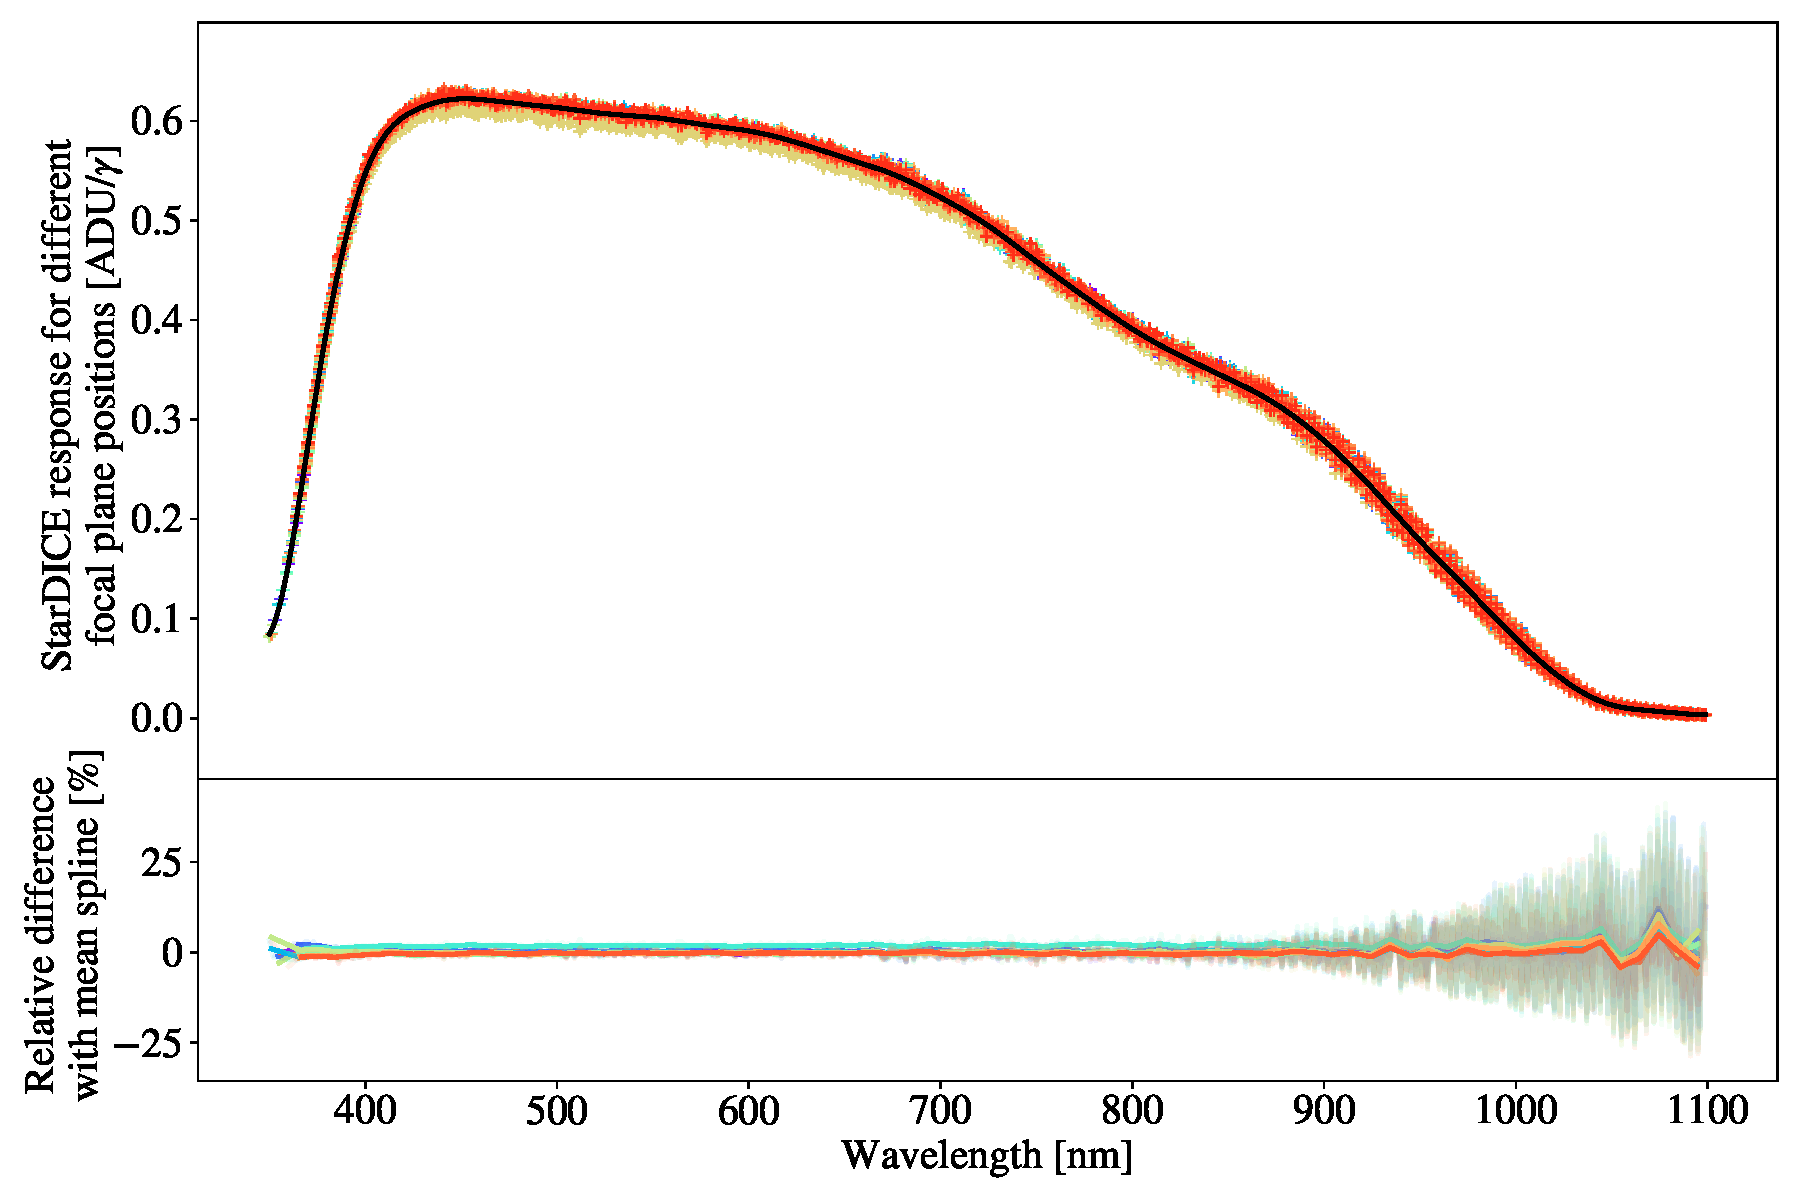
\includegraphics[width=\columnwidth]{fig/ccd_positions.pdf}
    \caption{Top : \SD response for the different positions on the focal plane, but same position on the mirror. Bottom : Relative difference between the data and the mean spline.}
    \label{fig:ccd_positions}
    %~/stardice/analysis/cbp_paper/golden_sample_analysis/dr2/2022_03_09_stardice_transmission_grid_auto.ipynb
\end{figure}

\subsection{Systematic uncertainties}
\label{sec:systematics}

\subsubsection{Stability of the StarDice responses}

\subsubsection{Gain and linearity}
\label{sec:gain}

Varying pinhole with StarDice, and CBP
Varying QSW but depending on result it falls into this subsection or the following

\subsubsection{Pinhole chromaticity}

\subsubsection{Pull distributions}

\subsubsection{Courbes de croissances}




